\documentclass[parskip=full]{scrartcl}
\usepackage[top=2.54cm, bottom=2.54cm, left=2.54cm, right=2.54cm]{geometry}
\usepackage[utf8]{inputenc} % use utf8 file encoding for TeX sources
\usepackage[T1]{fontenc}    % avoid garbled Unicode text in pdf
\usepackage[ngerman]{babel}  % german hyphenation, quotes, etc
\usepackage{hyperref}       % hyperlinks in document
\usepackage{glossaries}     % glossary 
\usepackage{enumerate}      % advanced enumeration
\usepackage[shortlabels]{enumitem}
\usepackage[dvipsnames]{xcolor}
\usepackage{graphicx}
\usepackage{caption}        % add captions
\usepackage{adjustbox}      % add adjustmentbox
\usepackage{csquotes}

% Set footer and header bar
\usepackage[headsepline, footsepline]{scrlayer-scrpage}
\addtokomafont{headsepline}{\color{BlueViolet}}
\addtokomafont{footsepline}{\color{BlueViolet}}
\KOMAoptions{headsepline=1.25pt:\textwidth}
\KOMAoptions{footsepline=1.25pt:\textwidth}
\clearpairofpagestyles
\rofoot{\thepage}
\ihead{Write your own Android App: SpiceSquad}

% set the hyperlink style in the document
\hypersetup{
    pdftitle={PSE: Entwurfsheft},
    pdfborderstyle={/S/U/W 1},
    colorlinks,
    linkcolor={black!50!black},
    citecolor={blue!50!black},
    urlcolor={blue!80!black}
}

% sets right quotation for "
\MakeOuterQuote{"}

%change figure numbering
\renewcommand{\thefigure}{\thesection.\arabic{figure}}

%add command to hide subsections from toc
\newcommand{\changelocaltocdepth}[1]{%
  \addtocontents{toc}{\protect\setcounter{tocdepth}{#1}}%
  \setcounter{tocdepth}{#1}%
}

\newcommand{\enablesubsectionnumbering}[1]{
    \renewcommand{\thesubsection}{$\langle$#1\arabic{subsection}0$\rangle$}
    \changelocaltocdepth{1} 
}

\newcommand{\resetsubsectionnumbering}{
    \renewcommand{\thesubsection}{\arabic{section}.\arabic{subsection}}
    \changelocaltocdepth{3} 
}

% glossary
\makeglossaries
\renewcommand{\glossarysection}[2][]{}

\begin{document}
\newglossaryentry{label}{
    name=Label,
    plural=Labels,
    description={Rezepte können mit bezeichnenden Stichwörtern, sogenannten Labels, versehen werden. Dies ermöglicht das Filtern von Rezepten nach bestimmten Eigenschaften (z.B. vegetarisch, glutenfrei, halal)}
}

\begin{titlepage}
    \begin{center}
        \begin{Huge}
            {\textbf{Write your own Android App: SpiceSquad}}
        \end{Huge}
        \vspace{12px}

        Praxis der Softwareentwicklung (PSE)\\
        Sommersemester 2023\\
        \vspace{150px}

        \begin{Huge}
            {\textbf{Entwurfsheft}}
        \end{Huge}
        \vspace{12px}

        \textbf{Auftraggeber}\\
        Karlsruher Institut für Technologie\\
        KASTEL — Institut für Informationssicherheit und Verlässlichkeit\\
        \vspace{330px}

        \textbf{Auftragnehmer}\\
        Karlsruher Intellektuelle\\
        Henri Becker, Konrad Knappe, Lukas Schwarz, Raphael Zipperer\\
    \end{center}
\end{titlepage}

\tableofcontents
\newpage

\section*{Gender-Hinweis}
Zur besseren Lesbarkeit wird in diesem Entwurfsheft das generische Maskulinum verwendet.
Die in diesem Heft verwendeten Personenbezeichnungen beziehen sich – sofern nicht anders kenntlich gemacht – auf alle Geschlechter.
\newpage

\section{Einleitung}
Das Entfurfsheft des Projekts: "Write your own Android App: SpiceSquad" baut auf dem zuvor verfassten Pflichtenheft auf.
Hierzu wurde zunächst ein umfassendes Klassendiagramm erstellt. Auf diesem basierend werden alle Klassen, Methoden und Attribute ausführlich erklärt.
In weiteren Kapiteln wird der REST-Webservice und die Datenbankstruktur beschrieben. Zum besseren Verständnis sind Ablaufbeschreibungen in Form von Sequenzdiagrammen angefügt.

\section{Struktur}

\subsection{Client-Server-Architektur}
Wie bereits im Pflichtenheft angeführt, haben wir uns für eine Trennung von Client und Server entschieden, um somit eine höchstmögliche Modularität zu gewährleisten und
Funktionen wie Squads zu ermöglichen. Die Kommunikation erfolgt über REST-Schnittstellen, welche eine einheitliche Schnittstelle mit dem Server bieten und eine einfache Skalierbarkeit ermöglichen.
Im Folgenden werden die Architekturen von Server und Client näher beschrieben.

\subsection{Architektur der Applikation}
Für die Entwicklung der Applikation soll Flutter benutzt werden. Dies bietet einige Vorteile. Flutter ist ein plattformübergreifendes Framework, das es Entwicklern ermöglicht, eine einzige Codebasis zu verwenden, um Apps sowohl für iOS als auch für Android zu erstellen. Dies reduziert den Entwicklungsaufwand erheblich, da Entwickler nicht separate Codes für jede Plattform schreiben müssen. Flutter verwendet die Dart-Programmiersprache, die eine einfache Syntax und eine umfangreiche Bibliothek bietet, um leistungsstarke und ansprechende Benutzeroberflächen zu erstellen. Darüber hinaus verfügt Flutter über eine Hot-Reload-Funktion, die es Entwicklern ermöglicht, Änderungen in Echtzeit zu sehen, was den Entwicklungsprozess beschleunigt. Flutter-Apps sind schnell, reaktionsfähig und bieten eine extrem gute Leistung, da sie direkt auf die nativen Funktionen des Betriebssystems zugreifen. Diese Kombination aus plattformübergreifender Entwicklung, einfacher Sprache, schnellem Entwicklungsprozess und guter Leistung macht Flutter zu einer guten Wahl für die Entwicklung von SpiceSquad.

Die Applikation wird in vier große Schichten gegliedert. Dies dient dazu, die Bestandteile der App nach ihrer Funktion zu gruppieren und die Abhängigkeiten zwischen den einzelnen Komponenten zu minimieren. Dadurch wird die Wartbarkeit massiv verbessert und auch die Erweiterbarkeit der Applikation wird durch diese Strukturierung erleichtert. Die Schichten orientieren sich stark an den Empfehlungen von Google für die Architektur von Android Applikationen. Die vier Schichten sind der \textbf{Presentation Layer}, der \textbf{Application Layer}, der \textbf{Domain Layer} und der \textbf{Data Layer}.
\begin{figure}[htp]
    \centering
    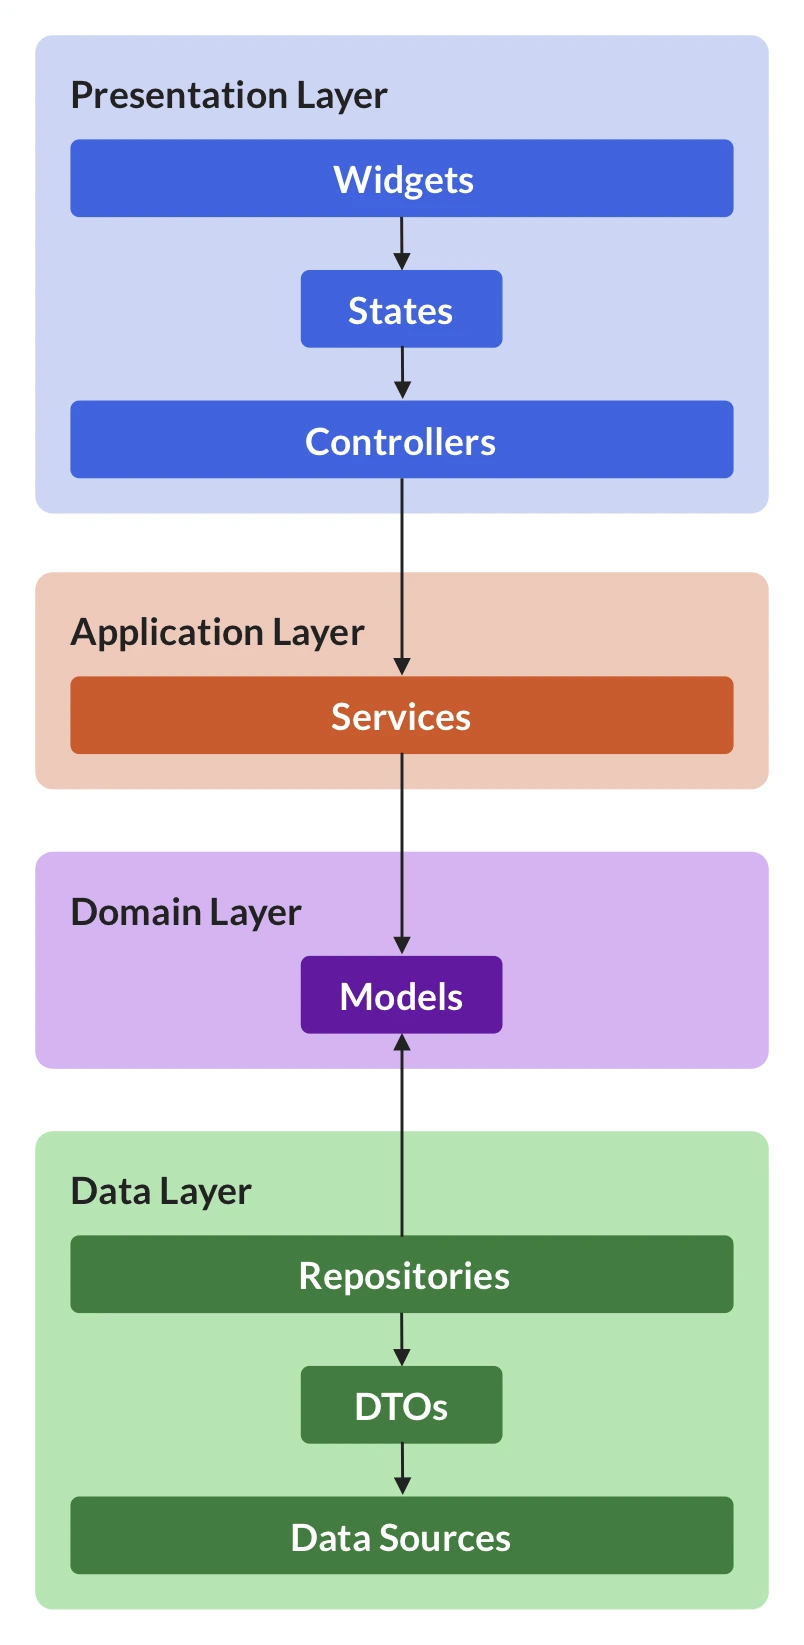
\includegraphics[height = 0.4\textheight]{images/architecture/architecture.png}
    \caption{Architektur der Applikation}
    \label{fig:struktur}
    %\footnotetext{Quelle: \url{https://codewithandrea.com/articles/flutter-app-architecture-application-layer/}}
\end{figure}
Die einzelnen Schichten werden in den folgenden Kapiteln genauer beschrieben.

\newpage

\changelocaltocdepth{2}

\section{Domain Layer}
Der Domain Layer enthält in erster Linie die Models der einzelnen Entitäten. Diese sollen nun genauer beschrieben werden. In den folgenden Klassendiagrammen wurden Getter der Übersicht halber weggelassen. Sie werden jedoch immer im Text beschrieben, sofern es sie gibt.
\begin{figure}[htp]
    \centering
    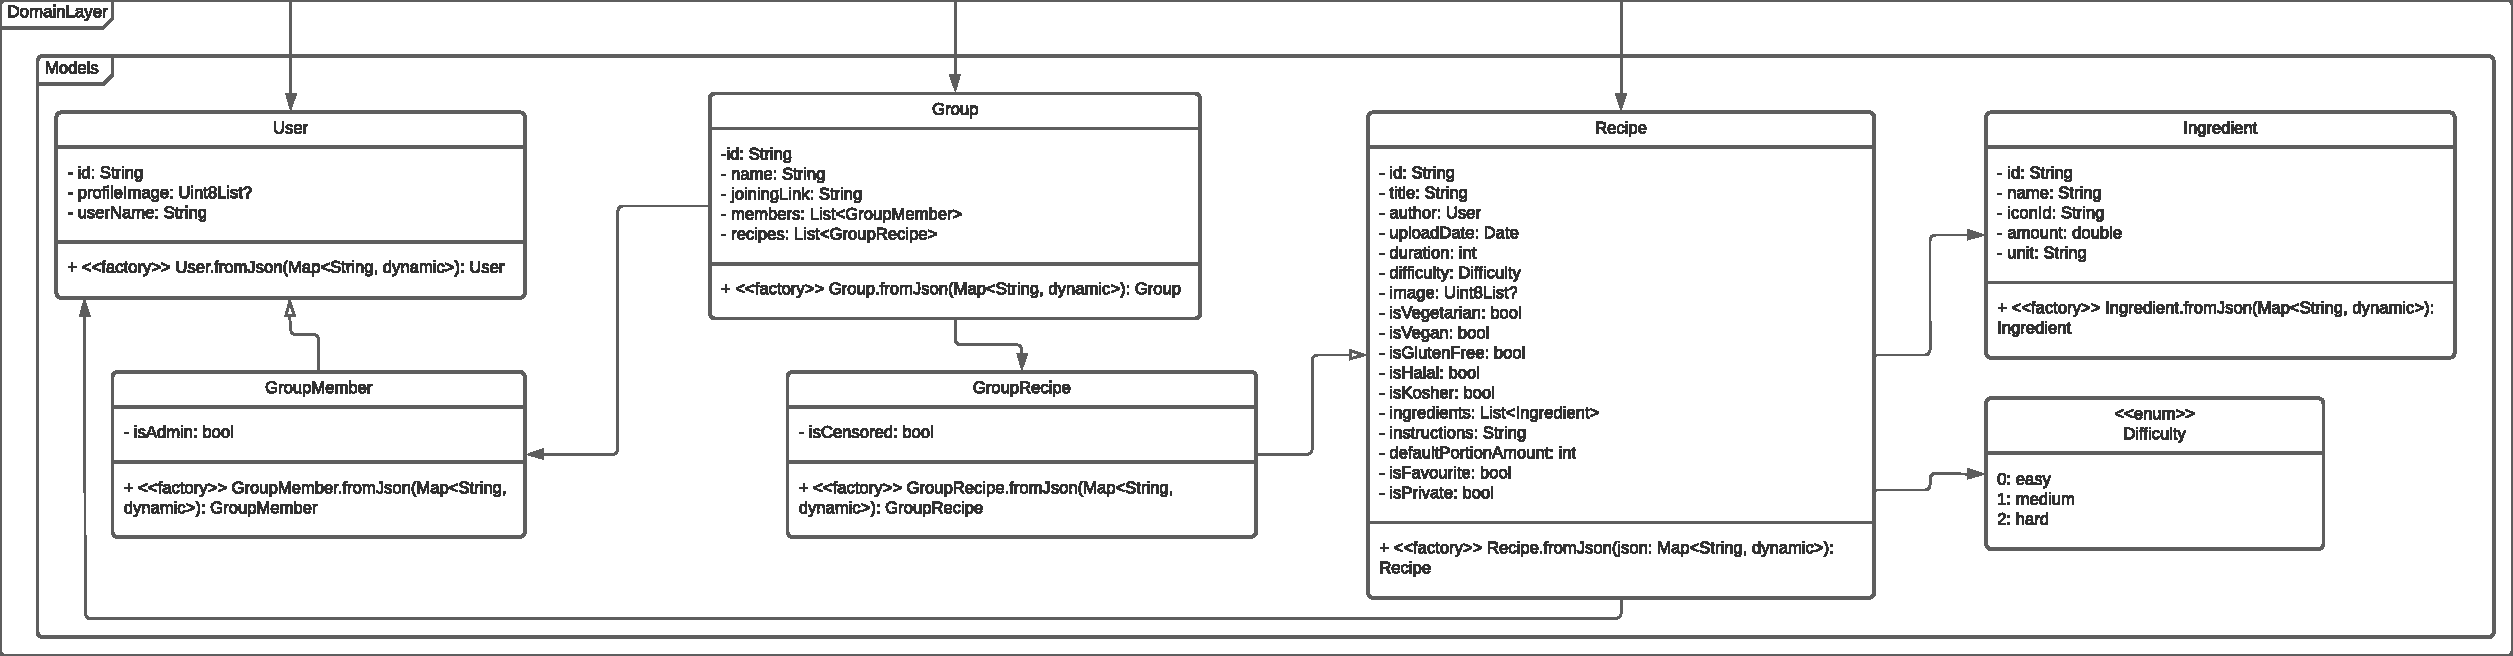
\includegraphics[width = \textwidth]{images/domainLayer/domainLayer.pdf}
    \caption{Klassendiagramm der Model-Klassen}
    \label{fig:domain-layer}
\end{figure}

\subsection{User}
Die User-Klasse repräsentiert einen Nutzer der App.
\subsubsection{Attribute}
Alle Attribute sind privat und können nur über einen Getter gelesen werden.
\paragraph{id: String}
Die eindeutige ID des Nutzers. Diese wird vom Server vergeben und ist somit nicht vom Nutzer selbst zu setzen.
\paragraph{profileImage: Uint8List?}
Das Profilbild des Nutzers. Der Typ Uint8List ist ein Array von Bytes, welches das Bild in binärer Form enthält. Dieses Attribut ist optional, da nicht jeder Nutzer ein Profilbild haben muss.
\paragraph{username: String}
Der Nutzername des Nutzers.

\subsubsection{Methoden}
\paragraph{getId(): String}
Gibt die ID des Nutzers zurück.
\paragraph{getProfileImage(): Uint8List?}
Gibt das Profilbild des Nutzers zurück. Ist kein Profilbild gesetzt, wird null zurückgegeben.
\paragraph{getUsername(): String}
Gibt den Nutzernamen des Nutzers zurück.
\paragraph{factory User.fromJson(Map<String, dynamic> json): User} Factory-Methode zum Erstellen eines User-Objekts aus einem \glslink{JSON}{JSON-Objekt}. Sie wird verwendet, um die Daten, die vom Server geschickt werden und in \Gls{JSON} vorliegen, in ein User-Objekt umzuwandeln. Die Methode ist statisch, da sie kein User-Objekt benötigt, um aufgerufen zu werden. Nimmt als Parameter das bereits in eine Map umgewandelte \glslink{JSON}{JSON-Objekt} entgegen und gibt ein User-Objekt zurück.

\subsection{Recipe}
Die Recipe-Klasse repräsentiert ein Rezept.
\subsubsection{Attribute}
Alle Attribute sind private und können nur über Getter-Methoden abgerufen werden.
\paragraph{id: String}
Die eindeutige ID des Rezepts. Diese wird vom Server vergeben und ist somit nicht vom Nutzer selbst zu setzen.
\paragraph{title: String}
Der Titel des Rezepts.
\paragraph{author: User}
Der Autor des Rezepts.
\paragraph{uploadDate: Date}
Das Datum, an dem das Rezept hochgeladen wurde.
\paragraph{duration: int}
Die Dauer zum Nachkochen des Rezepts in Minuten.
\paragraph{difficulty: Difficulty}
Die Schwierigkeit des Rezepts.
\paragraph{image: Uint8List?}
Das Bild des Rezepts. Der Typ Uint8List ist ein Array von Bytes, welches das Bild in binärer Form enthält. Dieses Attribut ist optional, da nicht jedes Rezept ein Bild haben muss.
\paragraph{isVegetartian: bool}
Gibt an, ob das Label "Vegetarisch" aktiviert ist.
\paragraph{isVegan: bool}
Gibt an, ob das Label "Vegan" aktiviert ist.
\paragraph{isGlutenFree: bool}
Gibt an, ob das Label "Glutenfrei" aktiviert ist.
\paragraph{isHalal: bool}
Gibt an, ob das Label "Halal" aktiviert ist.
\paragraph{isKosher: bool}
Gibt an, ob das Label "Koscher" aktiviert ist.
\paragraph{ingredients: List<Ingredient>}
Die Liste der Zutaten, die für das Rezept benötigt werden.
\paragraph{instructions: String}
Die Zubereitungsanleitung des Rezepts.
\paragraph{defaultPortionAmount: int}
Die Anzahl der Portionen, die das Rezept standardmäßig ergibt. Wird zum Berechnen der Mengen der Zutaten benötigt.
\paragraph{isFavourite: bool}
Gibt an, ob das Rezept vom Nutzer als Favorit markiert wurde.
\paragraph{isPrivate: bool}
Gibt an, ob das Rezept privat ist. Private Rezepte können nur vom Autor selbst gesehen werden.

\subsubsection{Methoden}
\paragraph{getId(): String}
Gibt die ID des Rezepts zurück.
\paragraph{getTitle(): String}
Gibt den Titel des Rezepts zurück.
\paragraph{getAuthor(): User}
Gibt den Autor des Rezepts zurück.
\paragraph{getUploadDate(): Date}
Gibt das Datum, an dem das Rezept hochgeladen wurde, zurück.
\paragraph{getDuration(): int}
Gibt die Dauer zum Nachkochen des Rezepts in Minuten zurück.
\paragraph{getDifficulty(): Difficulty}
Gibt die Schwierigkeit des Rezepts zurück.
\paragraph{getImage(): Uint8List?}
Gibt das Bild des Rezepts zurück. Ist kein Bild gesetzt, wird null zurückgegeben.
\paragraph{getIsVegetarian(): bool}
Gibt zurück, ob das Label "Vegetarisch" aktiviert ist.
\paragraph{getIsVegan(): bool}
Gibt zurück, ob das Label "Vegan" aktiviert ist.
\paragraph{getIsGlutenFree(): bool}
Gibt zurück, ob das Label "Glutenfrei" aktiviert ist.
\paragraph{getIsHalal(): bool}
Gibt zurück, ob das Label "Halal" aktiviert ist.
\paragraph{getIsKosher(): bool}
Gibt zurück, ob das Label "Koscher" aktiviert ist.
\paragraph{getIngredients(): List<Ingredient>}
Gibt die Liste der Zutaten, die für das Rezept benötigt werden, zurück.
\paragraph{getInstructions(): String}
Gibt die Zubereitungsanleitung des Rezepts zurück.
\paragraph{getDefaultPortionAmount(): int}
Gibt die Anzahl der Portionen, die das Rezept standardmäßig ergibt, zurück.
\paragraph{getIsFavourite(): bool}
Gibt zurück, ob das Rezept vom Nutzer als Favorit markiert wurde.
\paragraph{getIsPrivate(): bool}
Gibt zurück, ob das Rezept privat ist.
\paragraph{factory Recipe.fromJson(Map<String, dynamic> json): Recipe}
Factory-Methode zum Erstellen eines Recipe-Objekts aus einem \glslink{JSON}{JSON-Objekt}. Sie wird verwendet, um die Daten, die vom Server geschickt werden und in \Gls{JSON} vorliegen, in ein Recipe-Objekt umzuwandeln. Die Methode ist statisch, da sie kein Recipe-Objekt benötigt, um aufgerufen zu werden. Nimmt als Parameter das bereits in eine Map umgewandelte \glslink{JSON}{JSON-Objekt} entgegen und gibt ein Recipe-Objekt zurück.

\subsection{Ingredient}
Die Ingredient-Klasse repräsentiert eine Zutat, die einem Rezept zugeordnet ist.
\paragraph{id: String}
Die eindeutige ID der Zutat. Diese wird vom Server vergeben und ist somit nicht vom Nutzer selbst zu setzen.
\subsubsection{Attribute}
Alle Attribute sind private und können nur über Getter-Methoden abgerufen werden.
\paragraph{name: String}
Der Name der Zutat.
\paragraph{iconId: String}
Die Id des Icons, das der Zutat zugeordnet ist.
\paragraph{amount: double}
Die Menge der Zutat, die für das Rezept benötigt wird.
\paragraph{unit: String}
Die Einheit der Zutatenmenge.

\subsubsection{Methoden}
\paragraph{getId(): String}
Gibt die ID der Zutat zurück.
\paragraph{getName(): String}
Gibt den Namen der Zutat zurück.
\paragraph{getIconId(): String}
Gibt die Id des Icons, das der Zutat zugeordnet ist, zurück.
\paragraph{getAmount(): double}
Gibt die Menge der Zutat, die für das Rezept benötigt wird, zurück.
\paragraph{getUnit(): String}
Gibt die Einheit der Zutatenmenge zurück.
\paragraph{factory Ingredient.fromJson(Map<String, dynamic> json): Ingredient}
Factory-Methode zum Erstellen eines Ingredient-Objekts aus einem \glslink{JSON}{JSON-Objekt}. Sie wird verwendet, um die Daten, die vom Server geschickt werden und in \Gls{JSON} vorliegen, in ein Ingredient-Objekt umzuwandeln. Die Methode ist statisch, da sie kein Ingredient-Objekt benötigt, um aufgerufen zu werden. Nimmt als Parameter das bereits in eine Map umgewandelte \glslink{JSON}{JSON-Objekt} entgegen und gibt ein Ingredient-Objekt zurück.
\subsection{Difficulty}
Der Difficulty-Enum repräsentiert die Schwierigkeit eines Rezepts. Er kann folgende Werte annehmen:
\begin{itemize}
    \item easy
    \item medium
    \item hard
\end{itemize}

\subsection{Group}
Die Group-Klasse repräsentiert eine Gruppe bzw. Squad von Nutzern.
\subsubsection{Attribute}
Alle Attribute sind privat und können nur über einen Getter gelesen werden.
\paragraph{id: String}
Die eindeutige ID der Gruppe. Diese wird vom Server vergeben und ist somit nicht vom Nutzer selbst zu setzen.
\paragraph{name: String}
Der Name der Gruppe.
\paragraph{joiningLink: String}
Das Gruppenkürzel der Gruppe. Dieses wird verwendet, um einer Gruppe beizutreten.
\paragraph{members: List<GroupMember>}
Die Liste der Mitglieder der Gruppe. Die Liste ist nicht leer, da eine Gruppe mindestens einen Nutzer enthalten muss.
\paragraph{recipes: List<GroupRecipe>}
Die Liste der Rezepte, die von Mitgliedern der Gruppe erstellt wurden.

\subsubsection{Methoden}
\paragraph{getId(): String}
Gibt die ID der Gruppe zurück.
\paragraph{getName(): String}
Gibt den Namen der Gruppe zurück.
\paragraph{getJoiningLink(): String}
Gibt das Gruppenkürzel der Gruppe zurück.
\paragraph{getMembers(): List<GroupMember>}
Gibt die Liste der Mitglieder der Gruppe zurück.
\paragraph{getRecipes(): List<GroupRecipe>}
Gibt die Liste der Rezepte der Gruppe zurück.
\paragraph{factory Group.fromJson(Map<String, dynamic> json): Group} Factory-Methode zum Erstellen eines Group-Objekts aus einem \glslink{JSON}{JSON-Objekt}. Sie wird verwendet, um die Daten, die vom Server geschickt werden und in \Gls{JSON} vorliegen, in ein Group-Objekt umzuwandeln. Die Methode ist statisch, da sie kein Group-Objekt benötigt, um aufgerufen zu werden. Nimmt als Parameter das bereits in eine Map umgewandelte \glslink{JSON}{JSON-Objekt} entgegen und gibt ein Group-Objekt zurück.

\subsection{GroupMember}
Die GroupMember-Klasse repräsentiert ein Mitglied einer Gruppe. Sie erbt von der User-Klasse.
\subsubsection{Attribute}
Alle Attribute sind privat und können nur über einen Getter gelesen werden.
\paragraph{isAdmin: bool}
Gibt an, ob das Mitglied Administrator der Gruppe, der es zugeordnet ist, ist.
\subsubsection{Methoden}
\paragraph{getIsAdmin(): bool}
Gibt zurück, ob das Mitglied Administrator der Gruppe, der es zugeordnet ist, ist.
\paragraph{factory GroupMember.fromJson(Map<String, dynamic> json): GroupMember} Factory-Methode zum Erstellen eines GroupMember-Objekts aus einem \glslink{JSON}{JSON-Objekt}. Sie wird verwendet, um die Daten, die vom Server geschickt werden und in \Gls{JSON} vorliegen, in ein GroupMember-Objekt umzuwandeln. Die Methode ist statisch, da sie kein GroupMember-Objekt benötigt, um aufgerufen zu werden. Nimmt als Parameter das bereits in eine Map umgewandelte \glslink{JSON}{JSON-Objekt} entgegen und gibt ein GroupMember-Objekt zurück.

\subsection{GroupRecipe}
Die GroupRecipe-Klasse repräsentiert ein Rezept, das einer konkreten Gruppe zugeordnet wurde. Sie erbt von der Recipe-Klasse.
\subsubsection{Attribute}
Alle Attribute sind privat und können nur über einen Getter gelesen werden.
\paragraph{isCensored: bool}
Gibt an, ob das Rezept von einem Administrator der Gruppe zensiert wurde.
\subsubsection{Methoden}
\paragraph{getIsCensored(): bool}
Gibt zurück, ob das Rezept von einem Administrator der Gruppe zensiert wurde.
\paragraph{factory GroupRecipe.fromJson(Map<String, dynamic> json): GroupRecipe} Factory-Methode zum Erstellen eines GroupRecipe-Objekts aus einem \glslink{JSON}{JSON-Objekt}. Sie wird verwendet, um die Daten, die vom Server geschickt werden und in \Gls{JSON} vorliegen, in ein GroupRecipe-Objekt umzuwandeln. Die Methode ist statisch, da sie kein GroupRecipe-Objekt benötigt, um aufgerufen zu werden. Nimmt als Parameter das bereits in eine Map umgewandelte \glslink{JSON}{JSON-Objekt} entgegen und gibt ein GroupRecipe-Objekt zurück.

\section{Data Layer}
Der Data Layer ist für die Datenverarbeitung und -verwaltung verantwortlich. In der App selbst befinden sich lediglich die Repository-Klassen. Sie fungieren als eine Abstraktionsebene zwischen der Geschäftslogik (Application Layer) und den Datenquellen, wie z. B. einer lokalen Datenbank oder einem Remote-Server. Die Repository-Klassen bieten eine Schnittstelle, über die die Geschäftslogik auf die Daten zugreifen kann, ohne Details über deren Speicherung oder Beschaffung zu kennen. Sie bieten Methoden zur Datenabfrage, -aktualisierung und -speicherung und handhaben die Kommunikation mit den entsprechenden Datenquellen. Dadurch wird eine lose Kopplung zwischen der Geschäftslogik und den konkreten Datenquellen erreicht und ermöglicht eine flexiblere Handhabung von Datenquellenwechseln oder -aktualisierungen. Repository-Klassen unterstützen auch das Prinzip der Datenkapselung und fördern eine saubere und modularisierte Architektur in der App-Entwicklung.
Nun sollen die einzelnen Repository-Klassen vorgestellt werden. Die Klassen sind in Abbildung \ref{fig:dataLayer} dargestellt.
\begin{figure}[htp]
    \centering
    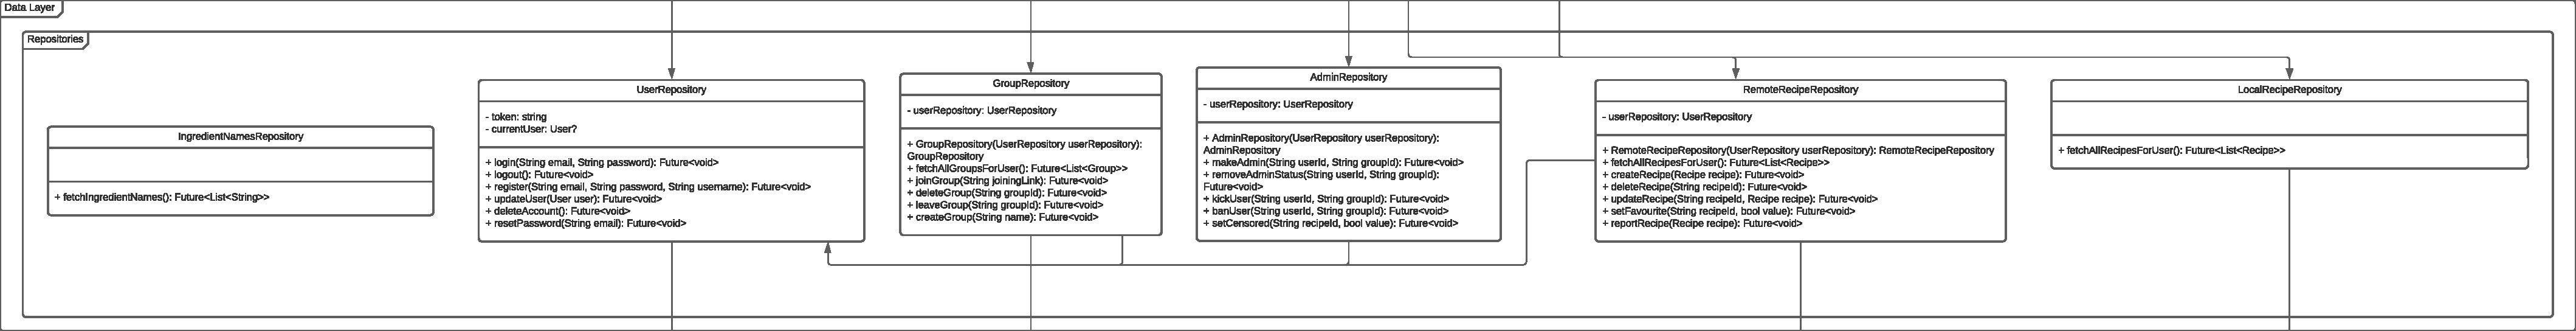
\includegraphics[width=\textwidth]{images/dataLayer/dataLayer.pdf}
    \caption{Klassendiagramm der Repository-Klassen}
    \label{fig:dataLayer}
\end{figure}

\subsection{UserRepository}
Das UserRepository stellt die Schnittstelle zwischen der Geschäftslogik und der Datenquelle für Nutzer dar. Es bietet Methoden zur Abfrage, Aktualisierung und Speicherung von Nutzern speichert das Token zur Authentifizierung des Nutzers bei dem Server.
\subsubsection{Attribute}
\paragraph{token: String}
Das Token zur Authentifizierung des Nutzers mit dem Server. Es handelt sich um ein privates Attribut, das nur über einen Getter gelesen werden kann. Das Token entspricht dem JWT-Token, das der Server nach der Authentifizierung des Nutzers zurückgibt. Darin sind unteranderem die Nutzer-ID und die Gültigkeitsdauer des Tokens kodiert enthalten.
\paragraph{currentUser: User}
Das User-Objekt, das den aktuell angemeldeten Nutzer repräsentiert. Es handelt sich um ein privates Attribut, das nur über einen Getter gelesen werden kann.
\subsubsection{Methoden}
\paragraph{getToken(): String}
Gibt das Token zur Authentifizierung des Nutzers bei dem Server zurück.
\paragraph{getCurrentUser(): User}
Gibt das User-Objekt, das den aktuell angemeldeten Nutzer repräsentiert, zurück.
\paragraph{login(String email, String password): Future<void>}
Es wird eine Anfrage zum Nutzer Anmelden an den Server gestellt. Nimmt als Parameter die E-Mail-Adresse und das Passwort des Nutzers entgegen. Die Methode ist asynchron und gibt ein Future-Objekt zurück. Das Future-Objekt wird aufgelöst, wenn die Anmeldung erfolgreich war. Wenn die Anmeldung fehlschlägt, wird eine Exception geworfen. Die Methode speichert das Token in dem privaten Attribut token und das User-Objekt, das den aktuell angemeldeten Nutzer repräsentiert, in dem privaten Attribut currentUser.
\paragraph{logout(): Future<void>}
Es wird eine Anfrage an den Server zum Abmelden des Nutzers gestellt. Die Methode ist asynchron und gibt ein Future-Objekt zurück. Das Future-Objekt wird aufgelöst, wenn die Abmeldung erfolgreich war. Wenn die Abmeldung fehlschlägt, wird eine Exception geworfen. Die Methode löscht das Token aus dem privaten Attribut token und das User-Objekt aus dem privaten Attribut currentUser.
\paragraph{register(String email, String password, String username): Future<void>}
Es wird eine Anfrage an den Server gestellt, einen neuen Nutzer zu registrieren. Nimmt als Parameter die E-Mail-Adresse, das Passwort und den Nutzernamen des Nutzers entgegen. Die Methode ist asynchron und gibt ein Future-Objekt zurück. Das Future-Objekt wird aufgelöst, wenn die Registrierung erfolgreich war. Wenn die Registrierung fehlschlägt, wird eine Exception geworfen. Die Methode speichert das Token in dem privaten Attribut token und das User-Objekt, das den aktuell angemeldeten Nutzer repräsentiert, in dem privaten Attribut currentUser.
\paragraph{updateUser(User user): Future<void>}
Es wird eine Anfrage an den Server gesendet, den angemeldeten Nutzer zu aktualisieren. Die Methode aktualisiert das User-Objekt, das den aktuell angemeldeten Nutzer repräsentiert, in dem privaten Attribut currentUser.
Die Methode ist asynchron und gibt ein Future-Objekt zurück. Das Future-Objekt wird aufgelöst, wenn die Anfrage erfolgreich war. Wenn die Anfrage fehlschlägt, wird eine Exception geworfen.
\paragraph{deleteAccount(): Future<void>}
Es wird eine Anfrage an den Server gesendet, um den Account des aktuell angemeldeten Nutzers zu löschen. Die Methode ist asynchron und gibt ein Future-Objekt zurück. Das Future-Objekt wird aufgelöst, wenn die Anfrage erfolgreich war. Wenn die Anfrage fehlschlägt, wird eine Exception geworfen. Die Methode führt im Anschluss die Methode logout() aus.
\paragraph{resetPassword(String email): Future<void>}
Es wird eine Anfrage an den Server zum Zurücksetzen des Passworts gesendet. Nimmt als Parameter die E-Mail-Adresse des Nutzers entgegen. Die Methode ist asynchron und gibt ein Future-Objekt zurück. Das Future-Objekt wird aufgelöst, wenn der Server eine E-Mail zum Zurücksetzen des Passworts versendet hat. Wenn das Versenden fehlschlägt, wird eine Exception geworfen.

\subsection{GroupRepository}
Das GroupRepository stellt die Schnittstelle zwischen der Geschäftslogik und der Datenquelle für Gruppen dar. Es bietet Methoden zur Abfrage, Aktualisierung und Speicherung von Gruppen.
\subsubsection{Attribute}
\paragraph{userRepository: UserRepository}
Das UserRepository-Objekt, das das GroupRepository-Objekt verwendet. Es handelt sich um ein privates Attribut. Es wird später verwendet, um das Token zur Authentifizierung des Nutzers bei dem Server für Anfragen zu erhalten.
\subsubsection{Methoden}
\paragraph{<<construtor>> GroupRepository(UserRepository userRepository): GroupRepository}
Konstruktor der Klasse. Initialisiert das Attribut userRepository mit dem übergebenen UserRepository-Objekt.
\paragraph{fetchAllGroupsForUser(): Future<List<Group>>}
Fragt alle Gruppen des angemeldeten Nutzers beim Server ab und gibt diese als Liste zurück. Die Methode ist asynchron und gibt ein Future-Objekt zurück. Das Future-Objekt wird aufgelöst, wenn die Abfrage erfolgreich war. Wenn die Abfrage fehlschlägt, wird eine Exception geworfen.
\paragraph{joinGroup(String joiningLink): Future<void>}
Es wird eine Anfrage an den Server zum Beitritt des aktuellen Nutzers zu einer Gruppe mit dem übergebenen Beitrittslink gestellt. Nimmt als Parameter den Beitrittslink der Gruppe entgegen. Die Methode ist asynchron und gibt ein Future-Objekt zurück. Das Future-Objekt wird aufgelöst, wenn der Nutzer erfolgreich der Gruppe beigetreten ist. Wenn der Nutzer der Gruppe nicht beitreten kann, wird eine Exception geworfen.
\paragraph{deleteGroup(String groupId): Future<void>}
Es wird eine Anfrage an den Server zum Löschen einer Gruppe mit der übergebenen Gruppen-ID gestellt. Nimmt als Parameter die ID der Gruppe entgegen. Die Methode ist asynchron und gibt ein Future-Objekt zurück. Das Future-Objekt wird aufgelöst, wenn die Gruppe erfolgreich gelöscht wurde. Wenn die Gruppe nicht gelöscht werden kann, wird eine Exception geworfen.
\paragraph{leaveGroup(String groupId): Future<void>}
Es wird eine Anfrage an den Server zum Austritt des aktuellen Nutzers aus einer Gruppe mit der übergebenen Gruppen-ID gestellt. Nimmt als Parameter die ID der Gruppe entgegen. Die Methode ist asynchron und gibt ein Future-Objekt zurück. Das Future-Objekt wird aufgelöst, wenn der Nutzer erfolgreich die Gruppe verlassen hat. Wenn der Nutzer die Gruppe nicht verlassen kann, wird eine Exception geworfen.
\paragraph{createGroup(String name): Future<void>}
Es wird eine Anfrage an den Server zum Erstellen einer neuen Gruppe mit dem übergebenen Namen gestellt. Nimmt als Parameter den Namen der Gruppe entgegen. Die Methode ist asynchron und gibt ein Future-Objekt zurück. Das Future-Objekt wird aufgelöst, wenn die Gruppe erfolgreich erstellt wurde. Wenn die Gruppe nicht erstellt werden kann, wird eine Exception geworfen.
\subsection{AdminRepository}
Das AdminRepository stellt die Schnittstelle zwischen der Geschäftslogik und den Server-Schnittstellen für verschiedene Administratoraktionen dar.
\subsubsection{Attribute}
\paragraph{userRepository: UserRepository}
Das UserRepository-Objekt, das das AdminRepository-Objekt verwendet. Es handelt sich um ein privates Attribut. Es wird später verwendet, um das Token zur Authentifizierung des Nutzers bei dem Server für Anfragen zu erhalten.
\subsubsection{Methoden}
\paragraph{<<construtor>> AdminRepository(UserRepository userRepository): AdminRepository}
Konstruktor der Klasse. Initialisiert das Attribut userRepository mit dem übergebenen UserRepository-Objekt.
\paragraph{makeAdmin(String userId, String groupId): Future<void>}
Es wird eine Anfrage an den Server gestellt, um den Nutzer mit der übergebenen ID zum Administrator der Gruppe mit der übergebenen ID zu machen. Nimmt als Parameter die ID des Nutzers und die ID der Gruppe entgegen. Die Methode ist asynchron und gibt ein Future-Objekt zurück. Das Future-Objekt wird aufgelöst, wenn der Nutzer erfolgreich zum Administrator der Gruppe gemacht wurde. Wenn der Nutzer nicht zum Administrator der Gruppe gemacht werden kann, wird eine Exception geworfen.

\paragraph{removeAdminStatus(String userId, String groupId): Future<void>}
Es wird eine Anfrage an den Server gestellt, um den Nutzer mit der übergebenen ID den Administratorstatus der Gruppe mit der übergebenen ID zu entziehen. Nimmt als Parameter die ID des Nutzers und die ID der Gruppe entgegen. Die Methode ist asynchron und gibt ein Future-Objekt zurück. Das Future-Objekt wird aufgelöst, wenn der Nutzer erfolgreich den Administratorstatus der Gruppe entzogen bekommen hat. Wenn der Nutzer nicht den Administratorstatus der Gruppe entzogen bekommen kann, wird eine Exception geworfen.
\paragraph{kickUser(String userId, String groupId): Future<void>}
Es wird eine Anfrage an den Server gestellt, um den Nutzer mit der übergebenen ID aus der Gruppe mit der übergebenen ID zu entfernen. Nimmt als Parameter die ID des Nutzers und die ID der Gruppe entgegen. Die Methode ist asynchron und gibt ein Future-Objekt zurück. Das Future-Objekt wird aufgelöst, wenn der Nutzer erfolgreich aus der Gruppe entfernt wurde. Wenn der Nutzer nicht aus der Gruppe entfernt werden kann, wird eine Exception geworfen.
\paragraph{banUser(String userId, String groupId): Future<void>}
Es wird eine Anfrage an den Server gestellt, um den Nutzer mit der übergebenen ID aus der Gruppe mit der übergebenen ID zu bannen. Nimmt als Parameter die ID des Nutzers und die ID der Gruppe entgegen. Die Methode ist asynchron und gibt ein Future-Objekt zurück. Das Future-Objekt wird aufgelöst, wenn der Nutzer erfolgreich aus der Gruppe gebannt wurde. Wenn der Nutzer nicht aus der Gruppe gebannt werden kann, wird eine Exception geworfen.
\paragraph{setCensored(String recipeId, bool value): Future<void>}
Setzt das Rezept mit der übergebenen ID als zensiert. Nimmt als Parameter die ID des Rezepts und einen boolschen Wert, der angibt, ob das Rezept als zensiert gesetzt oder entfernt werden soll, entgegen. Die Methode ist asynchron und gibt ein Future-Objekt zurück. Das Future-Objekt wird aufgelöst, wenn das Rezept erfolgreich als zensiert gesetzt oder entfernt wurde. Wenn das Rezept nicht als zensiert gesetzt oder entfernt werden kann, wird eine Exception geworfen.

\subsection{RemoteRecipeRepository}
Das RemoteRecipeRepository stellt die Schnittstelle zwischen der Geschäftslogik und den Server-Schnittstellen für Rezepte dar.
\subsubsection{Attribute}
\paragraph{userRepository: UserRepository}
Das UserRepository-Objekt, das das RemoteRecipeRepository-Objekt verwendet. Es handelt sich um ein privates Attribut. Es wird später verwendet, um das Token zur Authentifizierung des Nutzers bei dem Server für Anfragen zu erhalten.
\subsubsection{Methoden}
\paragraph{<<construtor>> RemoteRecipeRepository(UserRepository userRepository): RemoteRecipeRepository}
Konstruktor der Klasse. Initialisiert das Attribut userRepository mit dem übergebenen UserRepository-Objekt.
\paragraph{fetchRecipeById(String recipeId): Future<Recipe>}
Fragt das Rezept mit der übergebenen ID vom Server ab. Nimmt als Parameter die ID des Rezepts entgegen. Die Methode ist asynchron und gibt ein Future-Objekt zurück. Das Future-Objekt wird aufgelöst, wenn das Rezept erfolgreich vom Server abgefragt wurde. Wenn das Rezept nicht vom Server abgefragt werden kann, wird eine Exception geworfen.
\paragraph{fetchAllRecipesForUser(): Future<List<Recipe>>}
Fragt alle Rezepte aus Gruppen des aktuellen Nutzers vom Server ab. Nimmt keine Parameter entgegen. Die Methode ist asynchron und gibt ein Future-Objekt zurück. Das Future-Objekt wird aufgelöst, wenn die Rezepte erfolgreich vom Server abgefragt wurden. Wenn die Rezepte nicht vom Server abgefragt werden können, wird eine Exception geworfen. Speihert zudem alle Rezepte in den lokalen Speicher.
\paragraph{fetchOwnRecipes(): Future<List<Recipe>>}
Fragt alle Rezepte, die vom aktuellen Nutzer erstellt wurden, vom Server ab. Nimmt keine Parameter entgegen. Die Methode ist asynchron und gibt ein Future-Objekt zurück. Das Future-Objekt wird aufgelöst, wenn die Rezepte erfolgreich vom Server abgefragt wurden. Wenn die Rezepte nicht vom Server abgefragt werden können, wird eine Exception geworfen.
\paragraph{createRecipe(Recipe recipe): Future<void>}
Erstellt ein neues Rezept auf dem Server. Nimmt als Parameter das Rezept, das erstellt werden soll, entgegen. Die Methode ist asynchron und gibt ein Future-Objekt zurück. Das Future-Objekt wird aufgelöst, wenn das Rezept erfolgreich erstellt wurde. Wenn das Rezept nicht erstellt werden kann, wird eine Exception geworfen.
\paragraph{deleteRecipe(String recipeId): Future<void>}
Löscht das Rezept mit der übergebenen ID vom Server. Nimmt als Parameter die ID des Rezepts entgegen. Die Methode ist asynchron und gibt ein Future-Objekt zurück. Das Future-Objekt wird aufgelöst, wenn das Rezept erfolgreich gelöscht wurde. Wenn das Rezept nicht gelöscht werden kann, wird eine Exception geworfen.
\paragraph{updateRecipe(String recipeId, Recipe recipe): Future<void>}
Aktualisiert das Rezept mit der übergebenen ID auf dem Server. Nimmt als Parameter die ID des Rezepts und das aktualisierte Rezept entgegen. Die Methode ist asynchron und gibt ein Future-Objekt zurück. Das Future-Objekt wird aufgelöst, wenn das Rezept erfolgreich aktualisiert wurde. Wenn das Rezept nicht aktualisiert werden kann, wird eine Exception geworfen.
\paragraph{setFavourite(String recipeId, bool value): Futre<void>}
Setzt das Rezept mit der übergebenen ID als Favorit des aktuellen Nutzers. Nimmt als Parameter die ID des Rezepts und einen boolschen Wert, der angibt, ob das Rezept als Favorit gesetzt oder entfernt werden soll, entgegen. Die Methode ist asynchron und gibt ein Future-Objekt zurück. Das Future-Objekt wird aufgelöst, wenn das Rezept erfolgreich als Favorit gesetzt oder entfernt wurde. Wenn das Rezept nicht als Favorit gesetzt oder entfernt werden kann, wird eine Exception geworfen.

\subsection{LocalRecipeRepository}
Das LocalRecipeRepository stellt die Schnittstelle zwischen der Geschäftslogik und dem lokalen Speicher für Rezepte dar.
\subsubsection{Methoden}
\paragraph{fetchRecipeById(String recipeId): Future<Recipe>}
Fragt das Rezept mit der übergebenen ID aus dem lokalen Speicher ab. Nimmt als Parameter die ID des Rezepts entgegen. Die Methode ist asynchron und gibt ein Future-Objekt zurück. Das Future-Objekt wird aufgelöst, wenn das Rezept erfolgreich aus dem lokalen Speicher abgefragt wurde. Wenn das Rezept nicht aus dem lokalen Speicher abgefragt werden kann, wird eine Exception geworfen.
\paragraph{fetchAllRecipesForUser(): Future<List<Recipe>>}
Fragt alle Rezepte aus Gruppen des aktuellen Nutzers aus dem lokalen Speicher ab. Nimmt keine Parameter entgegen. Die Methode ist asynchron und gibt ein Future-Objekt zurück. Das Future-Objekt wird aufgelöst, wenn die Rezepte erfolgreich aus dem lokalen Speicher abgefragt wurden. Wenn die Rezepte nicht aus dem lokalen Speicher abgefragt werden können, wird eine Exception geworfen.
\paragraph{fetchOwnRecipes(): Future<List<Recipe>>}
Fragt alle Rezepte, die vom aktuellen Nutzer erstellt wurden, aus dem lokalen Speicher ab. Nimmt keine Parameter entgegen. Die Methode ist asynchron und gibt ein Future-Objekt zurück. Das Future-Objekt wird aufgelöst, wenn die Rezepte erfolgreich aus dem lokalen Speicher abgefragt wurden. Wenn die Rezepte nicht aus dem lokalen Speicher abgefragt werden können, wird eine Exception geworfen.

\section{Application Layer}
Der Application Layer ist eine weitere wichtige Komponente einer App. Seine Hauptaufgabe besteht darin, die Geschäftslogik der Anwendung zu implementieren und die Kernfunktionalität zu verwalten. Der Application Layer enthält verschiedene Klassen und Methoden, die die Regeln und Abläufe der Anwendung definieren. Er ist unabhängig von der Benutzeroberfläche und den spezifischen Details der Datenpersistenz. Stattdessen konzentriert sich der Application Layer darauf, die Kernfunktionalität der App zu modellieren und sicherzustellen, dass diese korrekt und effizient ausgeführt wird. Dadurch wird die Wiederverwendbarkeit, Testbarkeit und Flexibilität der Anwendung verbessert. Der Application Layer fungiert als Vermittler zwischen dem Presentation Layer und dem Data Layer und ermöglicht eine saubere Trennung der Verantwortlichkeiten in der App-Architektur. 
Er enthält in erster Linie viele verschiedene Services, die die verschiedenen Entitäten verwalten.
\begin{figure}[htp]
    \centering
    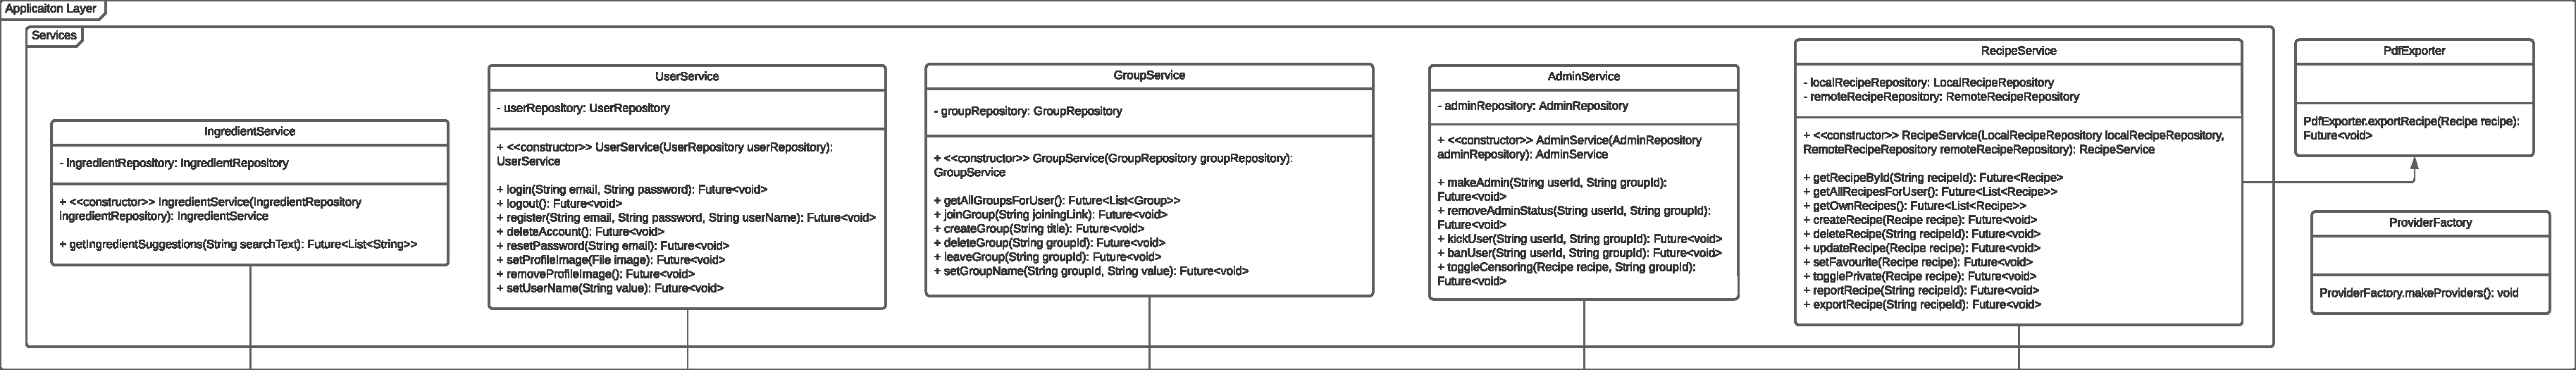
\includegraphics[width = \textwidth]{images/applicationLayer/applicationLayer.pdf}
    \caption{Klassendiagramm des Application Layer}
    \label{fig:application-layer}
\end{figure}

Nun werden die einzelnen Klassen des Application Layers beschrieben.

\subsection{IngredientService}
Der Service dient dazu, die Vorschläge für Zutatennamen zu finden und zu filtern.
\subsubsection{Attribute}
\paragraph{ingredientRepository: IngredientRepository}
Das IngredientRepository, das zum Zugriff auf die Zutatenvorschläge verwendet wird. Es wird im Konstruktor initialisiert und ist privat.
\subsubsection{Methoden}
\paragraph{<<constructor>> IngredientService(IngredientRepository ingredientRepository): IngredientService}
Konstruktor für den IngredientService. Initialisiert das IngredientRepository, das zum Zugriff auf die Zutatenvorschläge verwendet wird. Nimmt als Parameter das IngredientRepository entgegen.
\paragraph{getIngredientSuggestions(String searchText): Future<List<String>>}
Gibt eine Liste an Zeichenketten zurück, die Vorschläge für Zutatennamen darstellen. Nimmt als Parameter eine Zeichenkette entgegen, die die Suche nach Zutatennamen beschreibt. Die Methode ist asynchron und gibt ein Future-Objekt zurück. Das Future-Objekt wird aufgelöst, wenn die Vorschläge erfolgreich abgefragt wurden. Wenn die Vorschläge nicht abgefragt werden können, wird eine Exception geworfen. Die Methode ruft zum Zugriff auf die Zutatennamen eine Methode des IngredientRepository auf.

\subsection{UserService}
Der Service dient dazu, die Nutzer zu verwalten.
\subsubsection{Attribute}
\paragraph{userRepository: UserRepository}
Das UserRepository, das zum Zugriff auf die Nutzer verwendet wird. Es wird im Konstruktor initialisiert und ist privat.
\subsubsection{Methoden}
\paragraph{<<constructor>> UserService(UserRepository userRepository): UserService}
Konstruktor für den UserService. Initialisiert das UserRepository, das zum Zugriff auf die Nutzer verwendet wird. Nimmt als Parameter das UserRepository entgegen.
\paragraph{login(String email, String password): Future<void>}
Leitet die Loginanfrage an das zuständige Repository weiter. Nimmt als Parameter die E-Mail-Adresse und das Passwort des Nutzers entgegen. Die Methode ist asynchron und gibt ein Future-Objekt zurück. Das Future-Objekt wird aufgelöst, wenn der Nutzer erfolgreich eingeloggt wurde. Wenn der Nutzer nicht eingeloggt werden kann, wird eine Exception geworfen.
\paragraph{logout(): Future<void>}
Leitet die Logoutanfrage an das zuständige Repository weiter. Nimmt keine Parameter entgegen. Die Methode ist asynchron und gibt ein Future-Objekt zurück. Das Future-Objekt wird aufgelöst, wenn der Nutzer erfolgreich ausgeloggt wurde. Wenn der Nutzer nicht ausgeloggt werden kann, wird eine Exception geworfen.
\paragraph{register(String email, String password): Future<void>}
Leitet die Registrierungsanfrage an das zuständige Repository weiter. Nimmt als Parameter die E-Mail-Adresse und das Passwort des Nutzers entgegen. Die Methode ist asynchron und gibt ein Future-Objekt zurück. Das Future-Objekt wird aufgelöst, wenn der Nutzer erfolgreich registriert wurde. Wenn der Nutzer nicht registriert werden kann, wird eine Exception geworfen.
\paragraph{deleteAccount(): Future<void>}
Leitet die Anfrage zum Löschen des Nutzerkontos an das zuständige Repository weiter. Nimmt keine Parameter entgegen. Die Methode ist asynchron und gibt ein Future-Objekt zurück. Das Future-Objekt wird aufgelöst, wenn das Nutzerkonto erfolgreich gelöscht wurde. Wenn das Nutzerkonto nicht gelöscht werden kann, wird eine Exception geworfen.
\paragraph{resetPassword(String email): Future<void>}
Leitet die Anfrage zum Zurücksetzen des Passworts an das zuständige Repository weiter. Nimmt als Parameter die E-Mail-Adresse des Nutzers entgegen. Die Methode ist asynchron und gibt ein Future-Objekt zurück. Das Future-Objekt wird aufgelöst, wenn das Passwort erfolgreich zurückgesetzt wurde. Wenn das Passwort nicht zurückgesetzt werden kann, wird eine Exception geworfen.
\paragraph{setProfileImage(File image): Future<void>}
Leitet eine Anfrage zum Aktualisieren des Nutzers an das zuständige Repository weiter, indem ein Nutzer-Objekt mit verändertem Profilbild erzeugt wird. Nimmt als Parameter ein File-Objekt entgegen, das das neue Profilbild des Nutzers darstellt. Die Methode ist asynchron und gibt ein Future-Objekt zurück. Das Future-Objekt wird aufgelöst, wenn das Profilbild erfolgreich aktualisiert wurde. Wenn das Profilbild nicht aktualisiert werden kann, wird eine Exception geworfen.
\paragraph{removeProfileImage(): Future<void>}
Leitet eine Anfrage zum Aktualisieren des Nutzers an das zuständige Repository weite, indem ein Nutzer-Objekt ohne Profilbild erzeugt wird. Nimmt keine Parameter entgegen. Die Methode ist asynchron und gibt ein Future-Objekt zurück. Das Future-Objekt wird aufgelöst, wenn das Profilbild erfolgreich aktualisiert wurde. Wenn das Profilbild nicht aktualisiert werden kann, wird eine Exception geworfen.
\paragraph{setUserName(String value): Future<void>}
Leitet eine Anfrage zum Aktualisieren des Nutzers an das zuständige Repository weiter, indem ein Nutzer-Objekt mit verändertem Nutzernamen erzeugt wird. Nimmt als Parameter eine Zeichenkette entgegen, die den neuen Nutzernamen darstellt. Die Methode ist asynchron und gibt ein Future-Objekt zurück. Das Future-Objekt wird aufgelöst, wenn der Nutzername erfolgreich aktualisiert wurde. Wenn der Nutzername nicht aktualisiert werden kann, wird eine Exception geworfen.

\subsection{GroupService}
Der Service dient dazu, die Gruppen zu verwalten.
\subsubsection{Attribute}
\paragraph{groupRepository: GroupRepository}
Das GroupRepository, das zum Zugriff auf die Gruppen verwendet wird. Es wird im Konstruktor initialisiert und ist privat.
\subsubsection{Methoden}
\paragraph{<<constructor>> GroupService(GroupRepository groupRepository): GroupService}
Konstruktor für den GroupService. Initialisiert das GroupRepository, das zum Zugriff auf die Gruppen verwendet wird. Nimmt als Parameter das GroupRepository entgegen.
\paragraph{getAllGroupsForUser(): Future<List<Group>>}
Leitet die Anfrage zum Abrufen aller Gruppen, in denen der Nutzer Mitglied ist, an das zuständige Repository weiter. Nimmt keine Parameter entgegen. Die Methode ist asynchron und gibt ein Future-Objekt zurück. Das Future-Objekt wird aufgelöst, wenn die Gruppen erfolgreich abgerufen wurden. Wenn die Gruppen nicht abgerufen werden können, wird eine Exception geworfen.
\paragraph{joinGroup(String joiningLink): Future<void>}
Leitet die Anfrage zum Beitreten einer Gruppe an das zuständige Repository weiter. Nimmt als Parameter den Beitrete-Link der Gruppe entgegen. Die Methode ist asynchron und gibt ein Future-Objekt zurück. Das Future-Objekt wird aufgelöst, wenn der Nutzer erfolgreich der Gruppe beigetreten ist. Wenn der Nutzer nicht der Gruppe beitreten kann, wird eine Exception geworfen.
\paragraph{createGroup(String groupName): Future<void>}
Leitet die Anfrage zum Erstellen einer Gruppe an das zuständige Repository weiter. Nimmt als Parameter den Namen der Gruppe entgegen. Die Methode ist asynchron und gibt ein Future-Objekt zurück. Das Future-Objekt wird aufgelöst, wenn die Gruppe erfolgreich erstellt wurde. Wenn die Gruppe nicht erstellt werden kann, wird eine Exception geworfen.
\paragraph{deleteGroup(String groupId): Future<void>}
Leitet die Anfrage zum Löschen einer Gruppe an das zuständige Repository weiter. Nimmt als Parameter die ID der Gruppe entgegen. Die Methode ist asynchron und gibt ein Future-Objekt zurück. Das Future-Objekt wird aufgelöst, wenn die Gruppe erfolgreich gelöscht wurde. Wenn die Gruppe nicht gelöscht werden kann, wird eine Exception geworfen.
\paragraph{leaveGroup(String groupId): Future<void>}
Leitet die Anfrage zum Verlassen einer Gruppe an das zuständige Repository weiter. Nimmt als Parameter die ID der Gruppe entgegen. Die Methode ist asynchron und gibt ein Future-Objekt zurück. Das Future-Objekt wird aufgelöst, wenn der Nutzer erfolgreich die Gruppe verlassen hat. Wenn der Nutzer die Gruppe nicht verlassen kann, wird eine Exception geworfen.
\paragraph{setGroupName(String groupId, String groupName): Future<void>}
Leitet die Anfrage zum Aktualisieren einer Gruppe an das zuständige Repository weiter, indem ein neues Gruppen-Objekt mit aktualisiertem Namen erzeugt wird. Nimmt als Parameter die ID der Gruppe und den neuen Namen der Gruppe entgegen. Die Methode ist asynchron und gibt ein Future-Objekt zurück. Das Future-Objekt wird aufgelöst, wenn die Gruppe erfolgreich aktualisiert wurde. Wenn die Gruppe nicht aktualisiert werden kann, wird eine Exception geworfen.

\subsection{AdminService}
Der Service dient dazu, eine Schnittstelle für verschiedene Administratoraktionen bereitzustellen.
\subsubsection{Attribute}
\paragraph{adminRepository: AdminRepository}
Das AdminRepository, das zum Zugriff auf die Administratoraktionen verwendet wird. Es wird im Konstruktor initialisiert und ist privat.
\subsubsection{Methoden}
\paragraph{<<constructor>> AdminService(AdminRepository adminRepository): AdminService}
Konstruktor für den AdminService. Initialisiert das AdminRepository, das zum Zugriff auf die Administratoraktionen verwendet wird. Nimmt als Parameter das AdminRepository entgegen.
\paragraph{makeAdmin(String userId, String groupId): Future<void>}
Leitet die Anfrage zum Ernennen eines Nutzers zum Administrator einer Gruppe an das zuständige Repository weiter. Nimmt als Parameter die ID des Nutzers und die ID der Gruppe entgegen. Die Methode ist asynchron und gibt ein Future-Objekt zurück. Das Future-Objekt wird aufgelöst, wenn der Nutzer erfolgreich zum Administrator ernannt wurde. Wenn der Nutzer nicht zum Administrator ernannt werden kann, wird eine Exception geworfen.
\paragraph{removeAdminStatus(String userId, String groupId): Future<void>}
Leitet die Anfrage zum Entfernen des Administratorstatus eines Nutzers einer Gruppe an das zuständige Repository weiter. Nimmt als Parameter die ID des Nutzers und die ID der Gruppe entgegen. Die Methode ist asynchron und gibt ein Future-Objekt zurück. Das Future-Objekt wird aufgelöst, wenn der Administratorstatus des Nutzers erfolgreich entfernt wurde. Wenn der Administratorstatus des Nutzers nicht entfernt werden kann, wird eine Exception geworfen.
\paragraph{kickUser(String userId, String groupId): Future<void>}
Leitet die Anfrage zum Entfernen eines Nutzers aus einer Gruppe an das zuständige Repository weiter. Nimmt als Parameter die ID des Nutzers und die ID der Gruppe entgegen. Die Methode ist asynchron und gibt ein Future-Objekt zurück. Das Future-Objekt wird aufgelöst, wenn der Nutzer erfolgreich aus der Gruppe entfernt wurde. Wenn der Nutzer nicht aus der Gruppe entfernt werden kann, wird eine Exception geworfen.
\paragraph{banUser(String userId, String groupId): Future<void>}
Leitet die Anfrage zum Bannen eines Nutzers aus einer Gruppe an das zuständige Repository weiter. Nimmt als Parameter die ID des Nutzers und die ID der Gruppe entgegen. Die Methode ist asynchron und gibt ein Future-Objekt zurück. Das Future-Objekt wird aufgelöst, wenn der Nutzer erfolgreich aus der Gruppe gebannt wurde. Wenn der Nutzer nicht aus der Gruppe gebannt werden kann, wird eine Exception geworfen.
\paragraph{toggleCensoring(Recipe recipe, String groupId): Future<void>}
Leitet die Anfrage zum Aktivieren/Deaktivieren der Zensur eines Rezepts in einer Gruppe an das zuständige Repository weiter. Nimmt als Parameter das Rezept und die ID der Gruppe entgegen. Die Methode ist asynchron und gibt ein Future-Objekt zurück. Das Future-Objekt wird aufgelöst, wenn die Zensur des Rezepts erfolgreich geändert wurde. Wenn die Zensur des Rezepts nicht geändert werden kann, wird eine Exception geworfen.

\subsection{RecipeService}
Der Service dient dazu, die Rezepte zu verwalten.
\subsubsection{Attribute}
\paragraph{localRecipeRepository: LocalRecipeRepository}
Das Repository, das zum Zugriff auf die Rezepte im Systemspeicher verwendet wird. Es wird im Konstruktor initialisiert und ist privat. Besteht keine Verbindung zum Internet wird dieses Repository von den Methoden angesteuert.
\paragraph{remoteRecipeRepository: RemoteRecipeRepository}
Das Repository, das zum Zugriff auf die Rezepte in der Datenbank verwendet wird. Es wird im Konstruktor initialisiert und ist privat. Besteht eine Verbindung zum Internet wird dieses Repository von den Methoden angesteuert.
\subsubsection{Methoden}
\paragraph{<<constructor>> RecipeService(LocalRecipeRepository localRecipeRepository, RemoteRecipeRepository remoteRecipeRepository): RecipeService}
Konstruktor für den RecipeService. Initialisiert die Repositories, die zum Zugriff auf die Rezepte verwendet werden. Nimmt als Parameter das LocalRecipeRepository und das RemoteRecipeRepository entgegen.
\paragraph{getRecipeById(String recipeId): Future<Recipe>}
Leitet die Anfrage zum Abrufen eines Rezepts an das zuständige Repository weiter. Nimmt als Parameter die ID des Rezepts entgegen. Die Methode ist asynchron und gibt ein Future-Objekt zurück. Das Future-Objekt wird aufgelöst, wenn das Rezept erfolgreich abgerufen wurde. Wenn das Rezept nicht abgerufen werden kann, wird eine Exception geworfen.
\paragraph{getAllRecipesForUser(): Future<List<Recipe>>}
Leitet die Anfrage zum Abrufen aller Rezepte aus den Gruppen des Nutzers an das zuständige Repository weiter. Nimmt keine Parameter entgegen. Die Methode ist asynchron und gibt ein Future-Objekt zurück. Das Future-Objekt wird aufgelöst, wenn die Rezepte erfolgreich abgerufen wurden. Wenn die Rezepte nicht abgerufen werden können, wird eine Exception geworfen.
\paragraph{getOwnRecipes(): Future<List<Recipe>>}
Leitet die Anfrage zum Abrufen aller eigenen Rezepte des Nutzers an das zuständige Repository weiter. Nimmt keine Parameter entgegen. Die Methode ist asynchron und gibt ein Future-Objekt zurück. Das Future-Objekt wird aufgelöst, wenn die Rezepte erfolgreich abgerufen wurden. Wenn die Rezepte nicht abgerufen werden können, wird eine Exception geworfen.
\paragraph{createRecipe(Recipe recipe): Future<void>}
Leitet die Anfrage zum Erstellen eines Rezepts an das zuständige Repository weiter. Nimmt als Parameter das Rezept entgegen. Die Methode ist asynchron und gibt ein Future-Objekt zurück. Das Future-Objekt wird aufgelöst, wenn das Rezept erfolgreich erstellt wurde. Wenn das Rezept nicht erstellt werden kann, wird eine Exception geworfen.
\paragraph{deleteRecipe(String recipeId)}
Leitet die Anfrage zum Löschen eines Rezepts an das zuständige Repository weiter. Nimmt als Parameter die ID des Rezepts entgegen. Die Methode ist asynchron und gibt ein Future-Objekt zurück. Das Future-Objekt wird aufgelöst, wenn das Rezept erfolgreich gelöscht wurde. Wenn das Rezept nicht gelöscht werden kann, wird eine Exception geworfen.
\paragraph{updateRecipe(Recipe recipe): Future<void>}
Leitet die Anfrage zum Aktualisieren eines Rezepts an das zuständige Repository weiter. Nimmt als Parameter das Rezept mit den bereits aktualisierten Werten entgegen. Die Methode ist asynchron und gibt ein Future-Objekt zurück. Das Future-Objekt wird aufgelöst, wenn das Rezept erfolgreich aktualisiert wurde. Wenn das Rezept nicht aktualisiert werden kann, wird eine Exception geworfen.
\paragraph{toggleFavourite(Recipe recipe): Future<void>}
Leitet die Anfrage zum Aktivieren/Deaktivieren eines Rezepts als Favorit an das zuständige Repository weiter. Nimmt als Parameter das Rezept entgegen. Die Methode ist asynchron und gibt ein Future-Objekt zurück. Das Future-Objekt wird aufgelöst, wenn das Rezept erfolgreich als Favorit markiert wurde. Wenn das Rezept nicht als Favorit markiert werden kann, wird eine Exception geworfen.
\paragraph{togglePrivate(Recipe recipe): Future<void>}
Leitet die Anfrage zum Aktivieren/Deaktivieren eines Rezepts als privat an das zuständige Repository weiter. Nimmt als Parameter das Rezept entgegen. Die Methode ist asynchron und gibt ein Future-Objekt zurück. Das Future-Objekt wird aufgelöst, wenn das Rezept erfolgreich als privat markiert wurde. Wenn das Rezept nicht als privat markiert werden kann, wird eine Exception geworfen.
\paragraph{reportRecipe(String recipeId): Future<void>}
Leitet die Anfrage zum Melden eines Rezepts an das zuständige Repository weiter. Nimmt als Parameter die ID des Rezepts entgegen. Die Methode ist asynchron und gibt ein Future-Objekt zurück. Das Future-Objekt wird aufgelöst, wenn das Rezept erfolgreich gemeldet wurde. Wenn das Rezept nicht gemeldet werden kann, wird eine Exception geworfen.
\paragraph{exportRecipe(Recipe recipe): Future<void>}
Erstellt eine PDF-Datei mit Hilfe der PdfExporter-Klasse. Nimmt als Parameter das Rezept entgegen. Die Methode ist asynchron und gibt ein Future-Objekt zurück. Das Future-Objekt wird aufgelöst, wenn die PDF-Datei erfolgreich erstellt wurde. Wenn die PDF-Datei nicht erstellt werden kann, wird eine Exception geworfen.
\subsection{PdfExporter}
Der PdfExporter dient dazu, ein Template und Methoden zur Verfügung zu stellen, um ein Rezept als PDF-Datei zu exportieren.
\subsubsection{Methoden}
\paragraph{PdfExporter.exportRecipe(Recipe recipe): Future<void>}
Erstellt eine PDF-Datei, die das Rezept enthält und exportiert dieses anschließend. Nimmt als Parameter das Rezept entgegen. Die Methode ist asynchron und gibt ein Future-Objekt zurück. Das Future-Objekt wird aufgelöst, wenn die PDF-Datei erfolgreich erstellt und exportiert wurde. Wenn die PDF-Datei nicht erstellt und exportiert werden kann, wird eine Exception geworfen.
\subsection{ProviderFactory}
Die ProviderFactory dient dazu, die Riverpod-Provider zu erstellen. Mehr zu den Providern in \ref{sec:riverpod}.
\subsubsection{Methoden}
\paragraph{ProviderFactory.makeProviders(): void}
Legt alle Provider an, die für die Anwendung benötigt werden. Nimmt keine Parameter entgegen.
\newpage
\section{Presentation Layer}
\begin{figure}[htp]
    \centering
    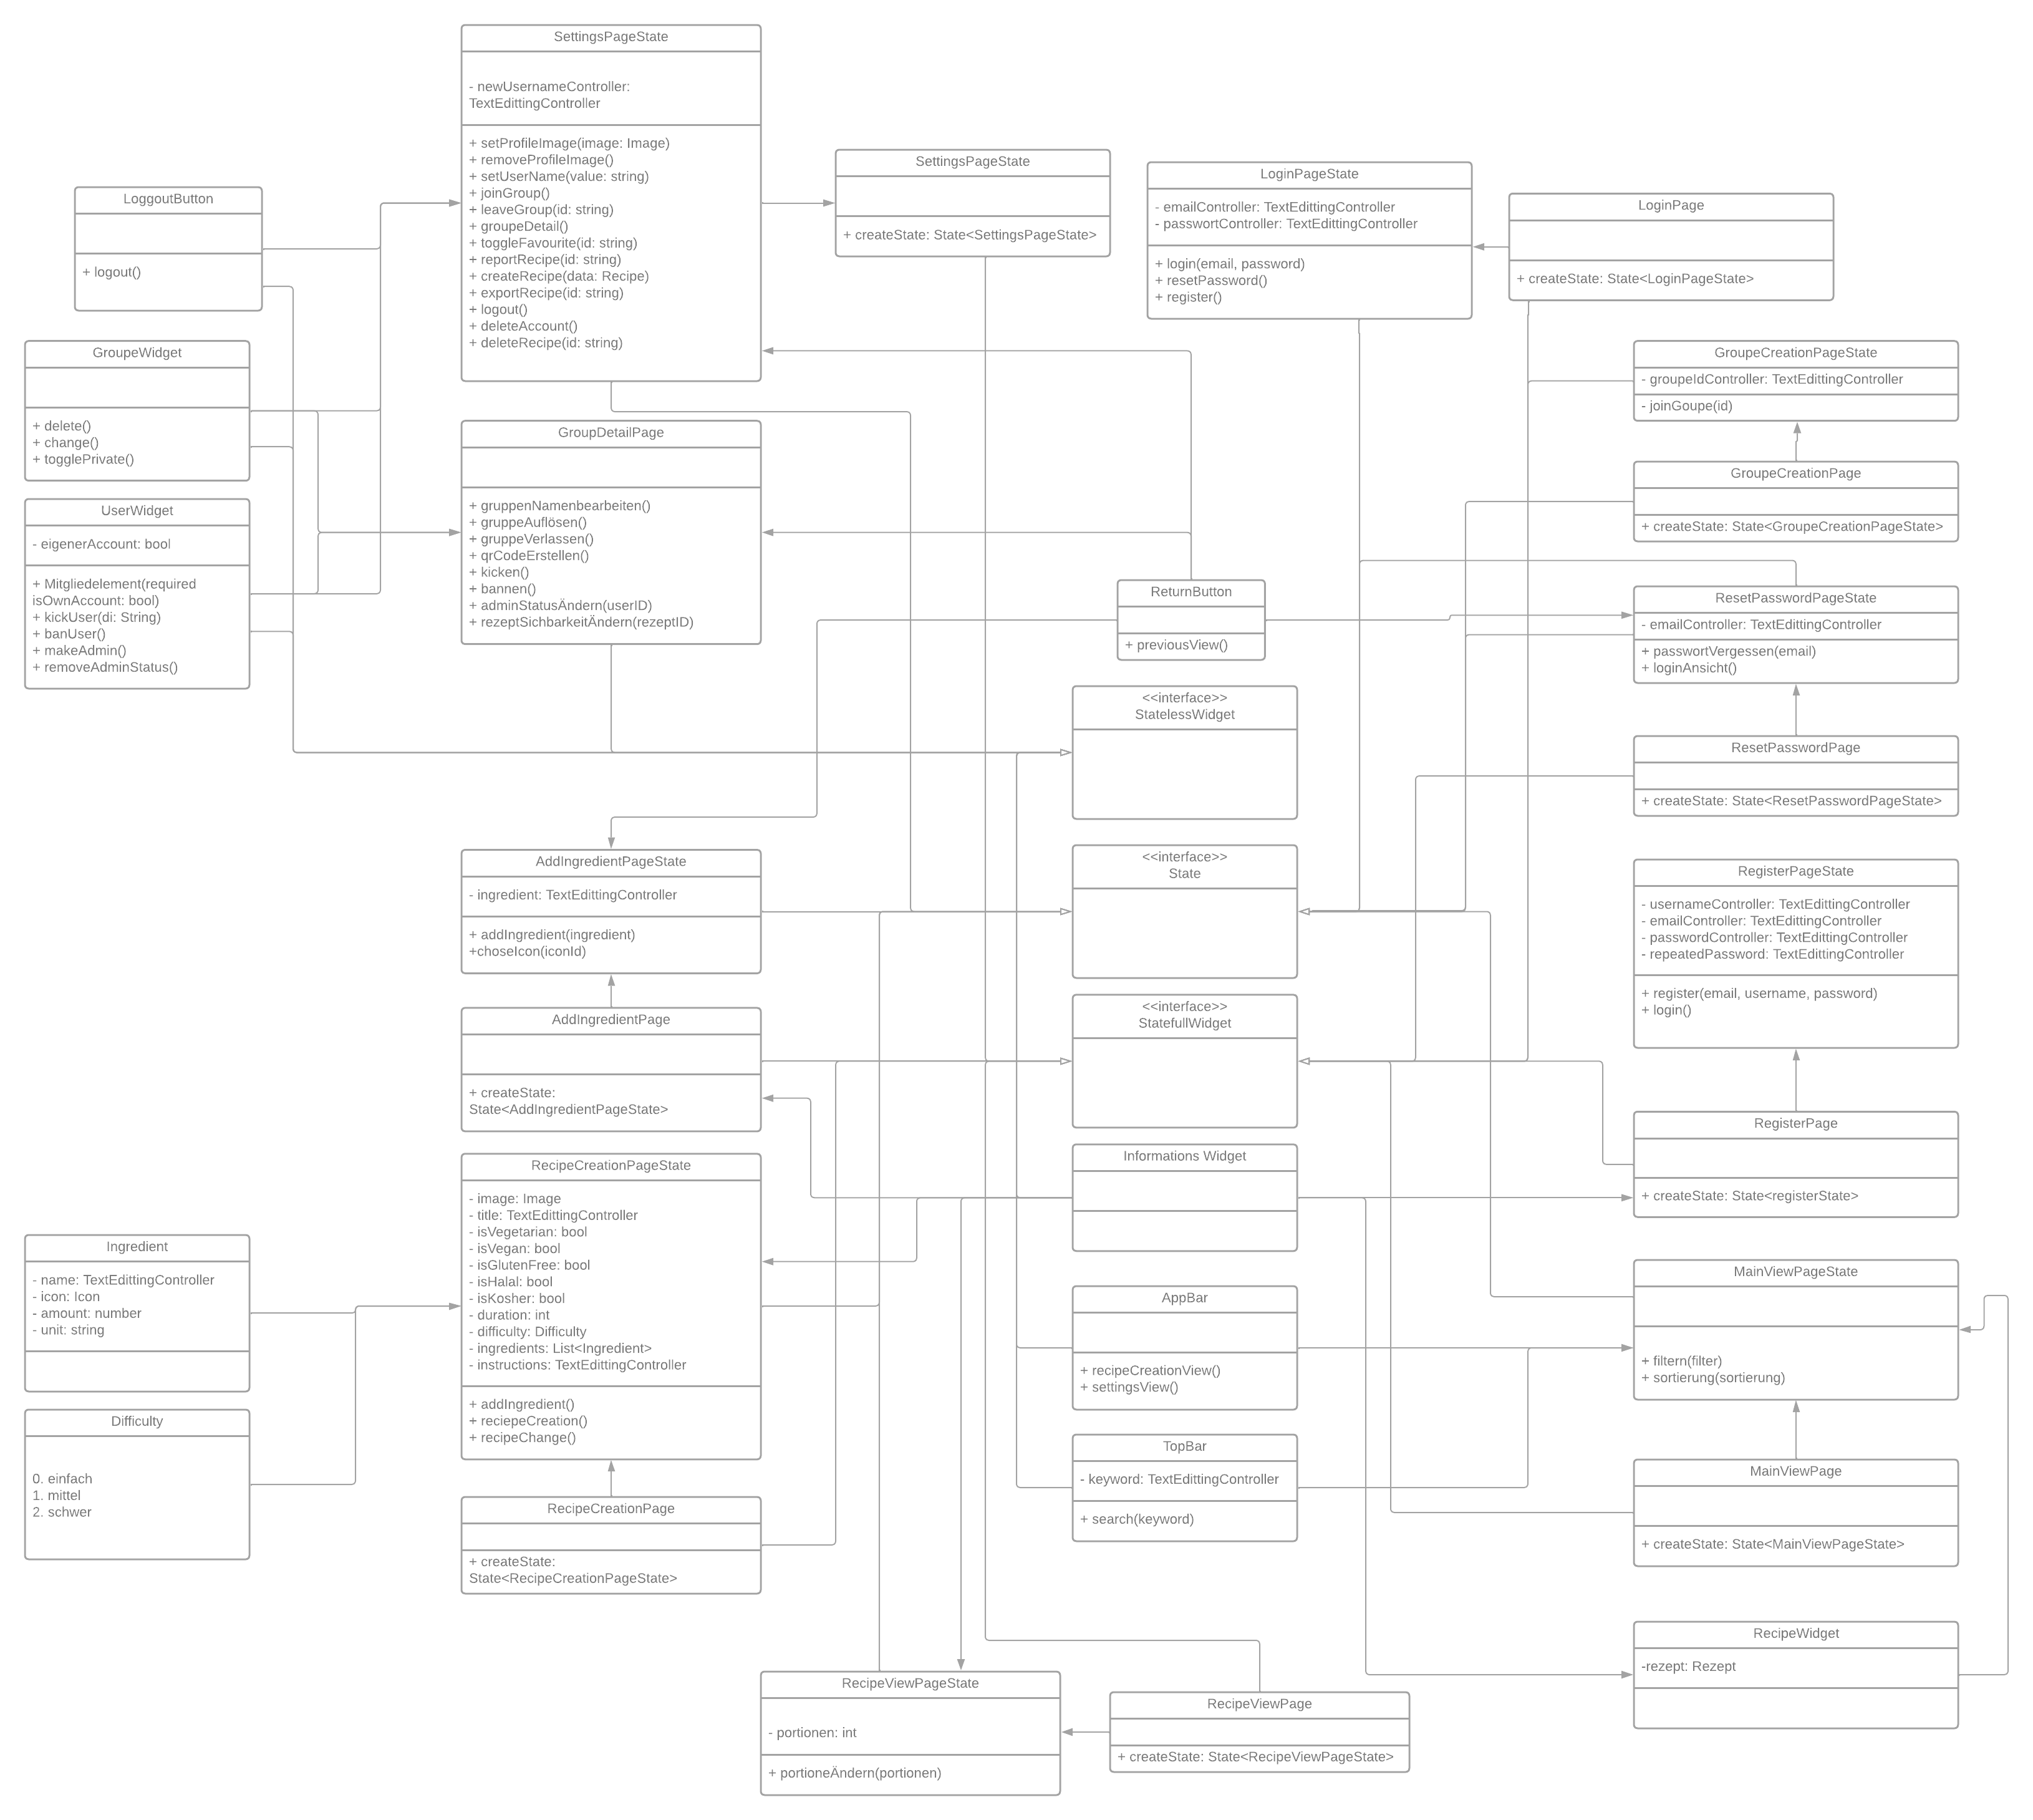
\includegraphics[width = \textwidth]{images/presentationLayer/presentationLayer.png}
    \caption{Klassendiagramm des Presentation Layer}
    \label{fig:presentation-layer}
\end{figure}

\newpage

\subsection{Hauptansicht}
    Die Klassen beinhaltet alle nötigen Funktionen und Attribute um die Hauptansicht darzustellen.

    \subsubsection{MainViewPage}
        \paragraph*{Methoden}
            \subparagraph*{createState: State<MainViewPageState>} - Konstruktor für den MainViewPageState.

    \subsubsection{MainViewPageState}
        \paragraph*{Methoden}

            \subparagraph*{filtering(filter: FilteringMethods)} - Alle Rezepte werden dem Filterkriterium gefiltert.
            \subparagraph*{sorting(sort: SortingMethods)} - Alle Rezepte werden nach dem Sortierkriterium sortiert.

    \subsubsection{TopBar}
        \paragraph*{Attribute}
            \subparagraph*{keyword: TextEdittingController} - Durch den Nutzer eingegebene Zeichenkette für die Suche.

        \paragraph*{Methode}
            \subparagraph*{ search(keyword: TextEdittingController)} - Durchsucht alle Rezepte und gibt die aus, deren Rezepttitel zu dem Schlagwort passen.

    \subsubsection{AppBar}
        \paragraph*{Methoden}
            \subparagraph*{recipeCreationView()} - Die Rezept-erstell-Ansicht wird aufgerufen.
            \subparagraph*{settingsView()} - Die Einstellungsansicht wird aufgerufen.

    \subsubsection{RecipeWidget}
        \paragraph*{Attribut}
            \subparagraph*{recipe: Recipe} - Das mit dem Widget dargestellte Rezept.

        \paragraph*{Methode}
            \subparagraph*{RecipeWidget(recipe: Recipe - notNull)} - Konstruktor für ein Recipe Widget. Ein Rezept muss angegeben werden.

    \subsubsection{InformationWidget} \label{sec:InformationWidget}
        \paragraph*{Attribute}
            \subparagraph*{information: InformationKategories} - Gibt an welche Information in dem Widget dargestellt werden soll.
            \subparagraph*{text: string} - Der Text der in dem Widget angezeigt werden kann.

        \paragraph*{Methoden}
            \subparagraph*{InformationWidget(information: InformationKategories - notNull, text: string)} - Konstruktor für ein Information Widget. Eine Information Kategorie muss angegeben werden.

    \subsubsection{SortingMethods}
        Ein Enum der alle Sortierung Methoden beinhält.
        \paragraph*{Content}
            \subparagraph*{alphabetical} - Die Rezepte werden alphabetisch sortiert.
            \subparagraph*{difficulty} - Die Rezepte werden nach dem \gls{schwierigkeit}{Schwierigkeitsgrad} sortiert.
            \subparagraph*{date} - Die Rezepte werden nach dem Hinzufüge Datum sortiert.

    \subsubsection{FilteringMehods}
        Ein Enum der alle Filter Methoden beinhält.
        \paragraph*{Content}
            \subparagraph*{favorites} - Die Rezepte werden nach Favoriten gefiltert.
            \subparagraph*{difficultyEasy} - Die Rezepte werden nach dem \glslink{schwierigkeit}{Schwierigkeitsgrad} einfach gefiltert.
            \subparagraph*{difficultyMedium} - Die Rezepte werden nach dem \glslink{schwierigkeit}{Schwierigkeitsgrad} mittel gefiltert.
            \subparagraph*{difficultyHard} - Die Rezepte werden nach dem \glslink{schwierigkeit}{Schwierigkeitsgrad} schwer gefiltert.
            \subparagraph*{labelVegetarian} - Die Rezepte werden nach dem \gls{label} vegetarisch gefiltert.
            \subparagraph*{labelVegan} - Die Rezepte werden nach dem \gls{label} vegan gefiltert.
            \subparagraph*{labelGlutenFree} - Die Rezepte werden nach dem \gls{label} glutenfrei gefiltert.
            \subparagraph*{labelHalal} - Die Rezepte werden nach dem \gls{label} halal gefiltert.
            \subparagraph*{labelKoscher} - Die Rezepte werden nach dem \gls{label} koscher gefiltert.

    \subsubsection{InformationKategories} \label{sec:InformationKategories}
        Ein Enum der alle Information Kategorien beinhält.
        \paragraph*{Content}
            \subparagraph*{duration} - Das Widget gibt die Zubereitungsdauer an.
            \subparagraph*{difficultyEasy} - Das Widget gibt den \glslink{schwierigkeit}{Schwierigkeitsgrad} einfach an.
            \subparagraph*{difficultyMedium} - Das Widget gibt den \glslink{schwierigkeit}{Schwierigkeitsgrad} mittel an.
            \subparagraph*{difficultyHard} - Das Widget gibt den \glslink{schwierigkeit}{Schwierigkeitsgrad} schwer an.
            \subparagraph*{labelVegetarian} - Das Widget gibt das \gls{label} vegetarisch an.
            \subparagraph*{labelVegan} - Das Widget gibt das \gls{label} vegan an.
            \subparagraph*{labelGlutenFree} - Das Widget gibt das \gls{label} Gluten frei an.
            \subparagraph*{labelHalal} - Das Widget gibt das \gls{label} halal an.
            \subparagraph*{labelKoscher} - Das Widget gibt das \gls{label} koscher an.

    \begin{figure}[htp]
        \begin{minipage}
            [t]{0.49\textwidth}
            \centering
            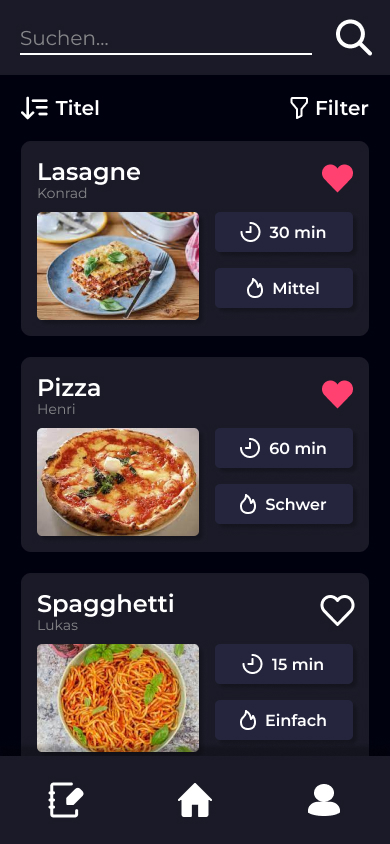
\includegraphics[height=80mm]{images/Presentation-layer/MainView.jpg}
            \caption{Hauptansicht}
        \end{minipage}
        \begin{minipage}
            [t]{0.49\textwidth}
            \centering
            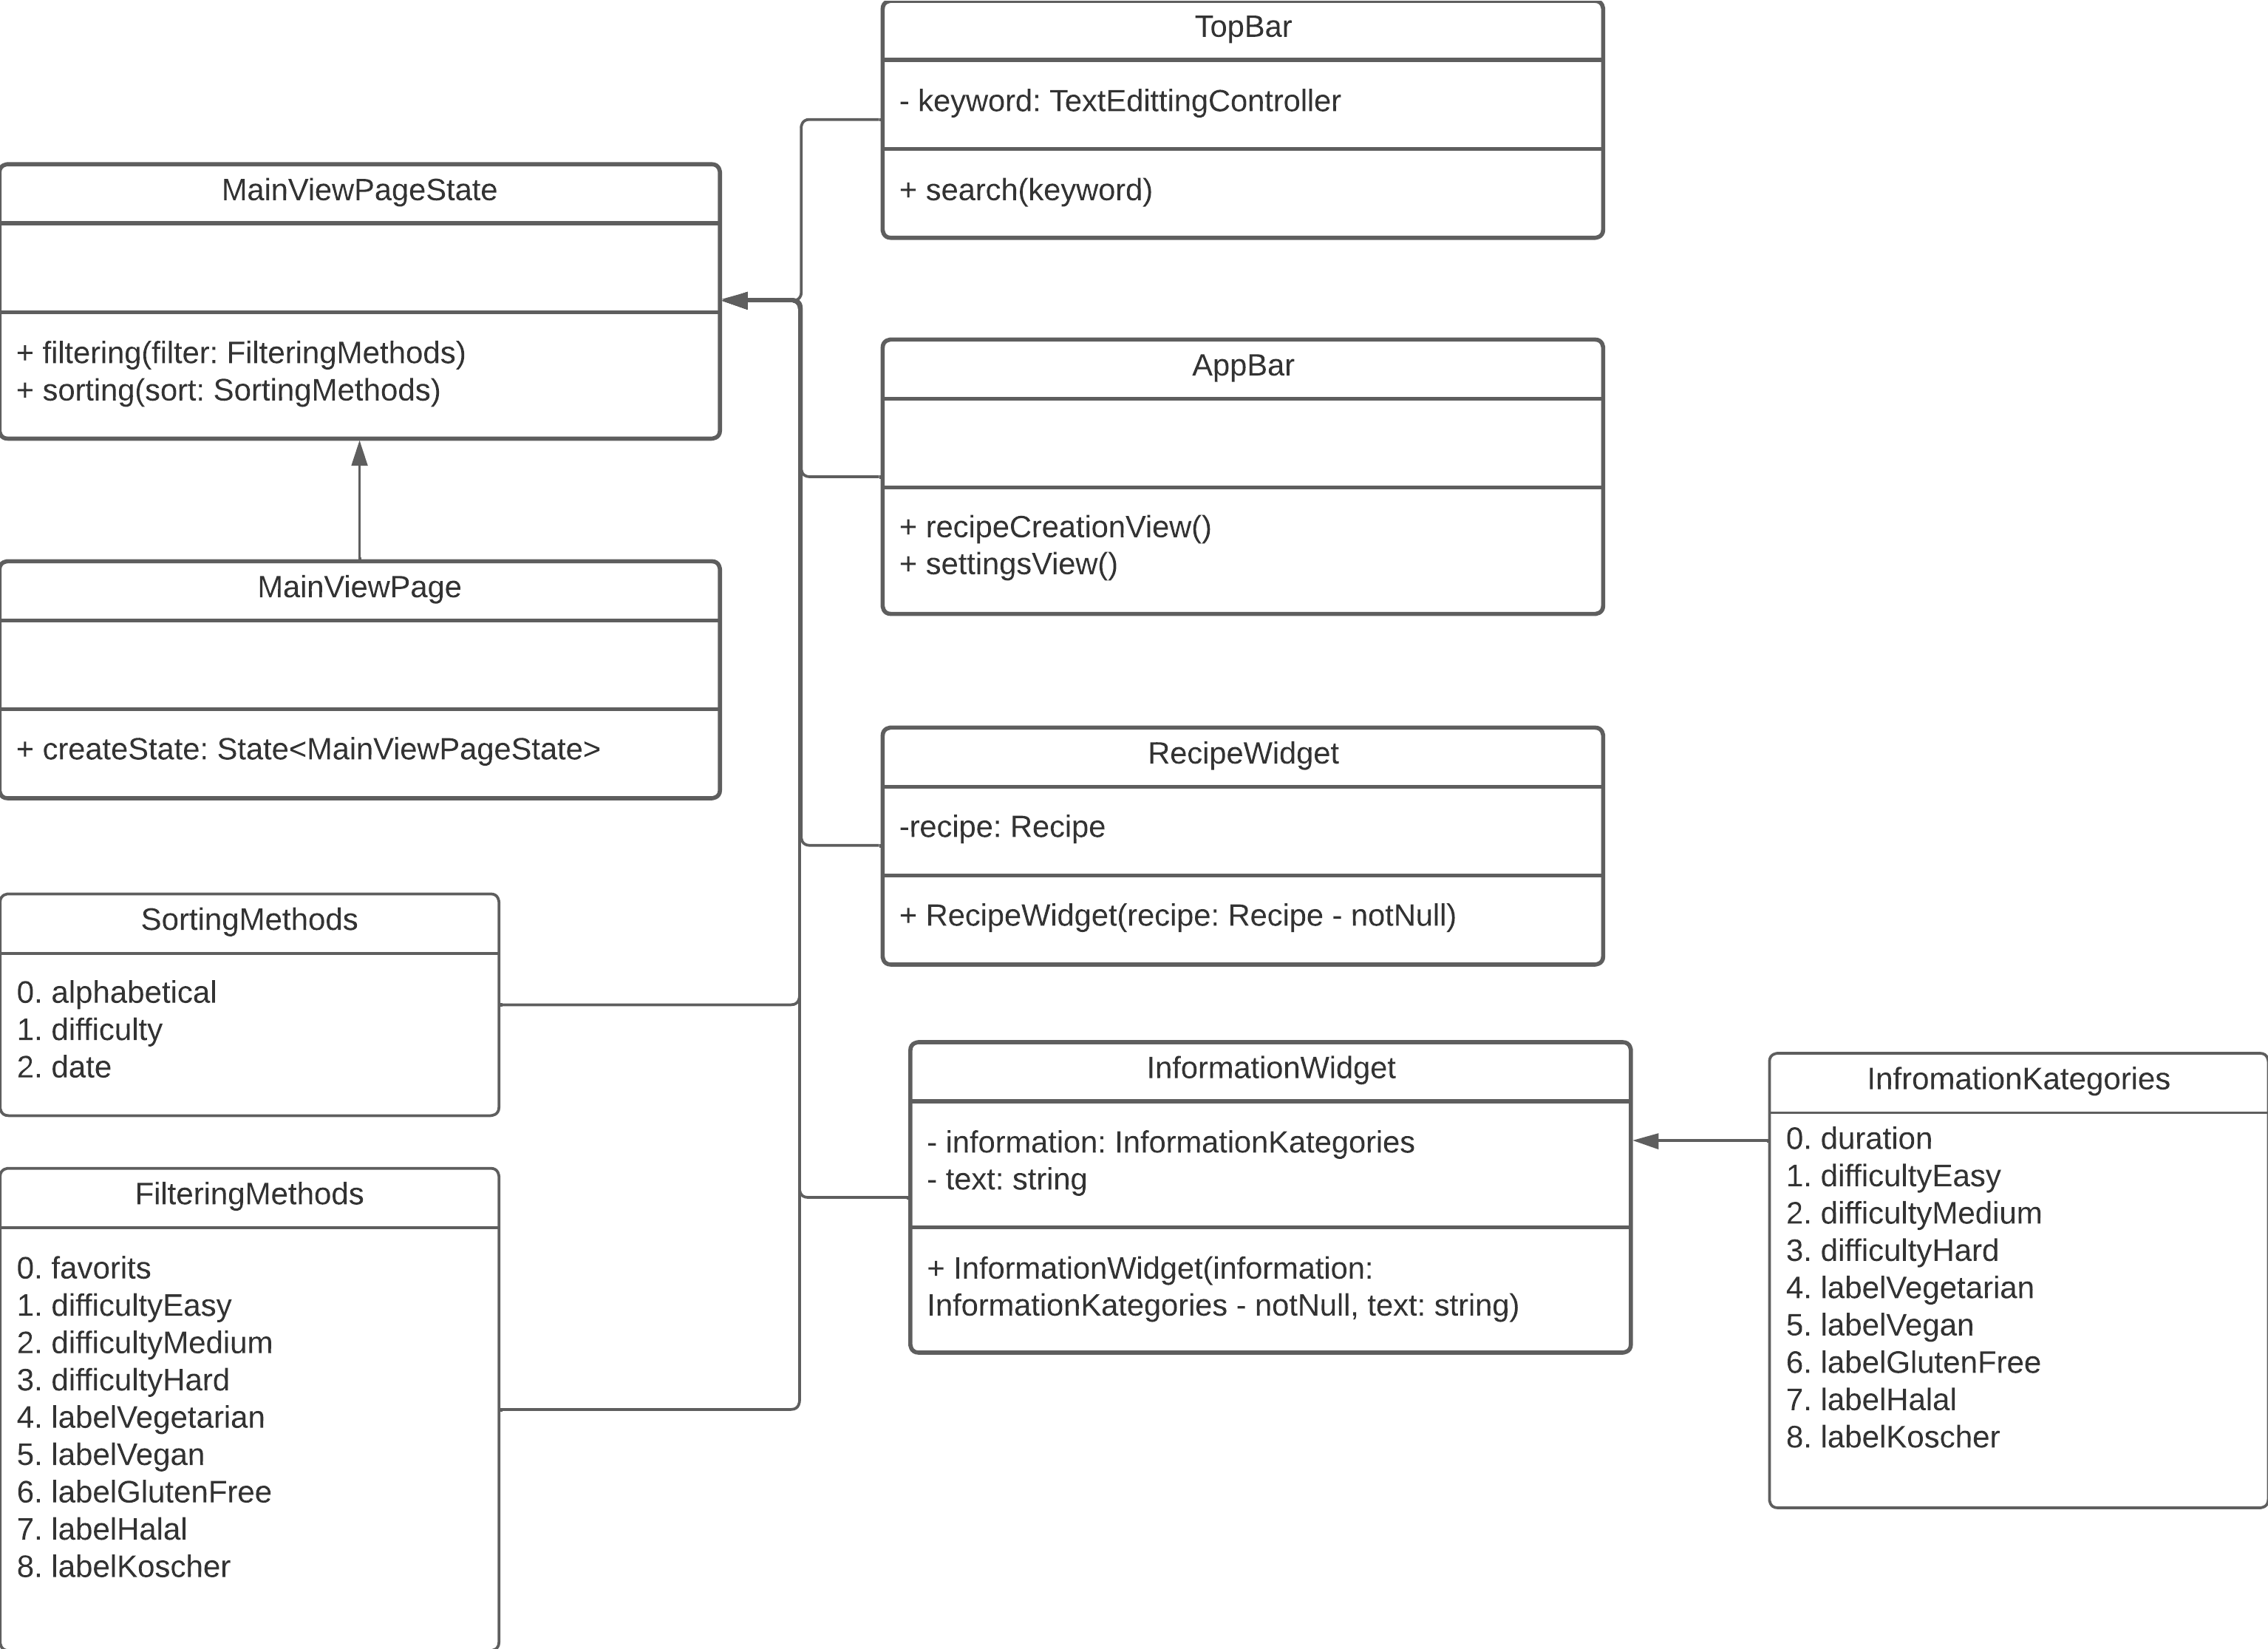
\includegraphics[width=0.95\textwidth]{images/Presentation-layer/MainViewClass.png}
            \caption{Klassen für Hauptansicht}
        \end{minipage}
    \end{figure}

\subsection{Rezeptansicht}
    Die Klassen beinhalten alle nötigen Funktionen und Attribute um die Hauptansicht darzustellen.

    \subsubsection{RecipeViewPage}
        \paragraph*{Methode}
            \subparagraph*{createState: State<RecipeViewPageState>} - Konstruktor für den RecipeViewPageState.
        
    \subsubsection{recipeViewPageState}
        \paragraph*{Attribut}
            \subparagraph*{portions: TextEdittingController} - Eingegebene Ganzzahl für die die Zutatenmengen berechnet werden. Ist standardmäßig auf der Portionsgröße die beim Rezepterstellen angegeben worden ist.
    
        \paragraph*{Method}
            \subparagraph*{changePortions(portions: int)} - Die neuen Mengenangaben für die Zutaten werden berechnet.

    \subsubsection{InformationWidget (\autoref{sec:InformationWidget})}

    \subsubsection{InformationKategories (\autoref{sec:InformationKategories})}

    \begin{figure}[htp]
        \begin{minipage}
            [t]{0.49\textwidth}
            \centering
            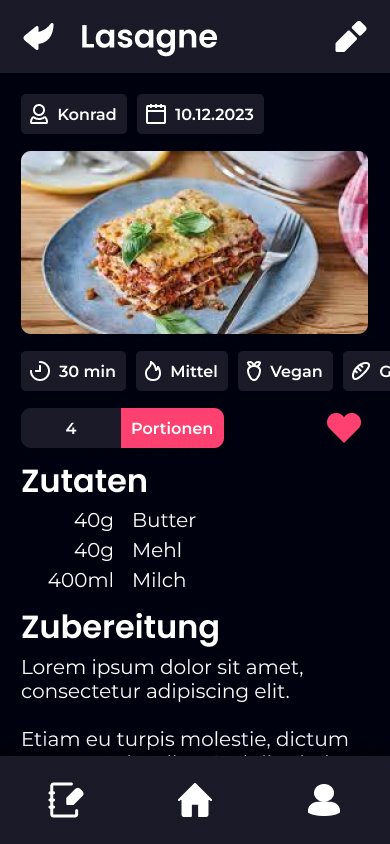
\includegraphics[height=80mm]{images/Presentation-layer/RecipeView.jpg}
            \caption{Rezeptansicht}
        \end{minipage}
        \begin{minipage}
            [t]{0.49\textwidth}
            \centering
            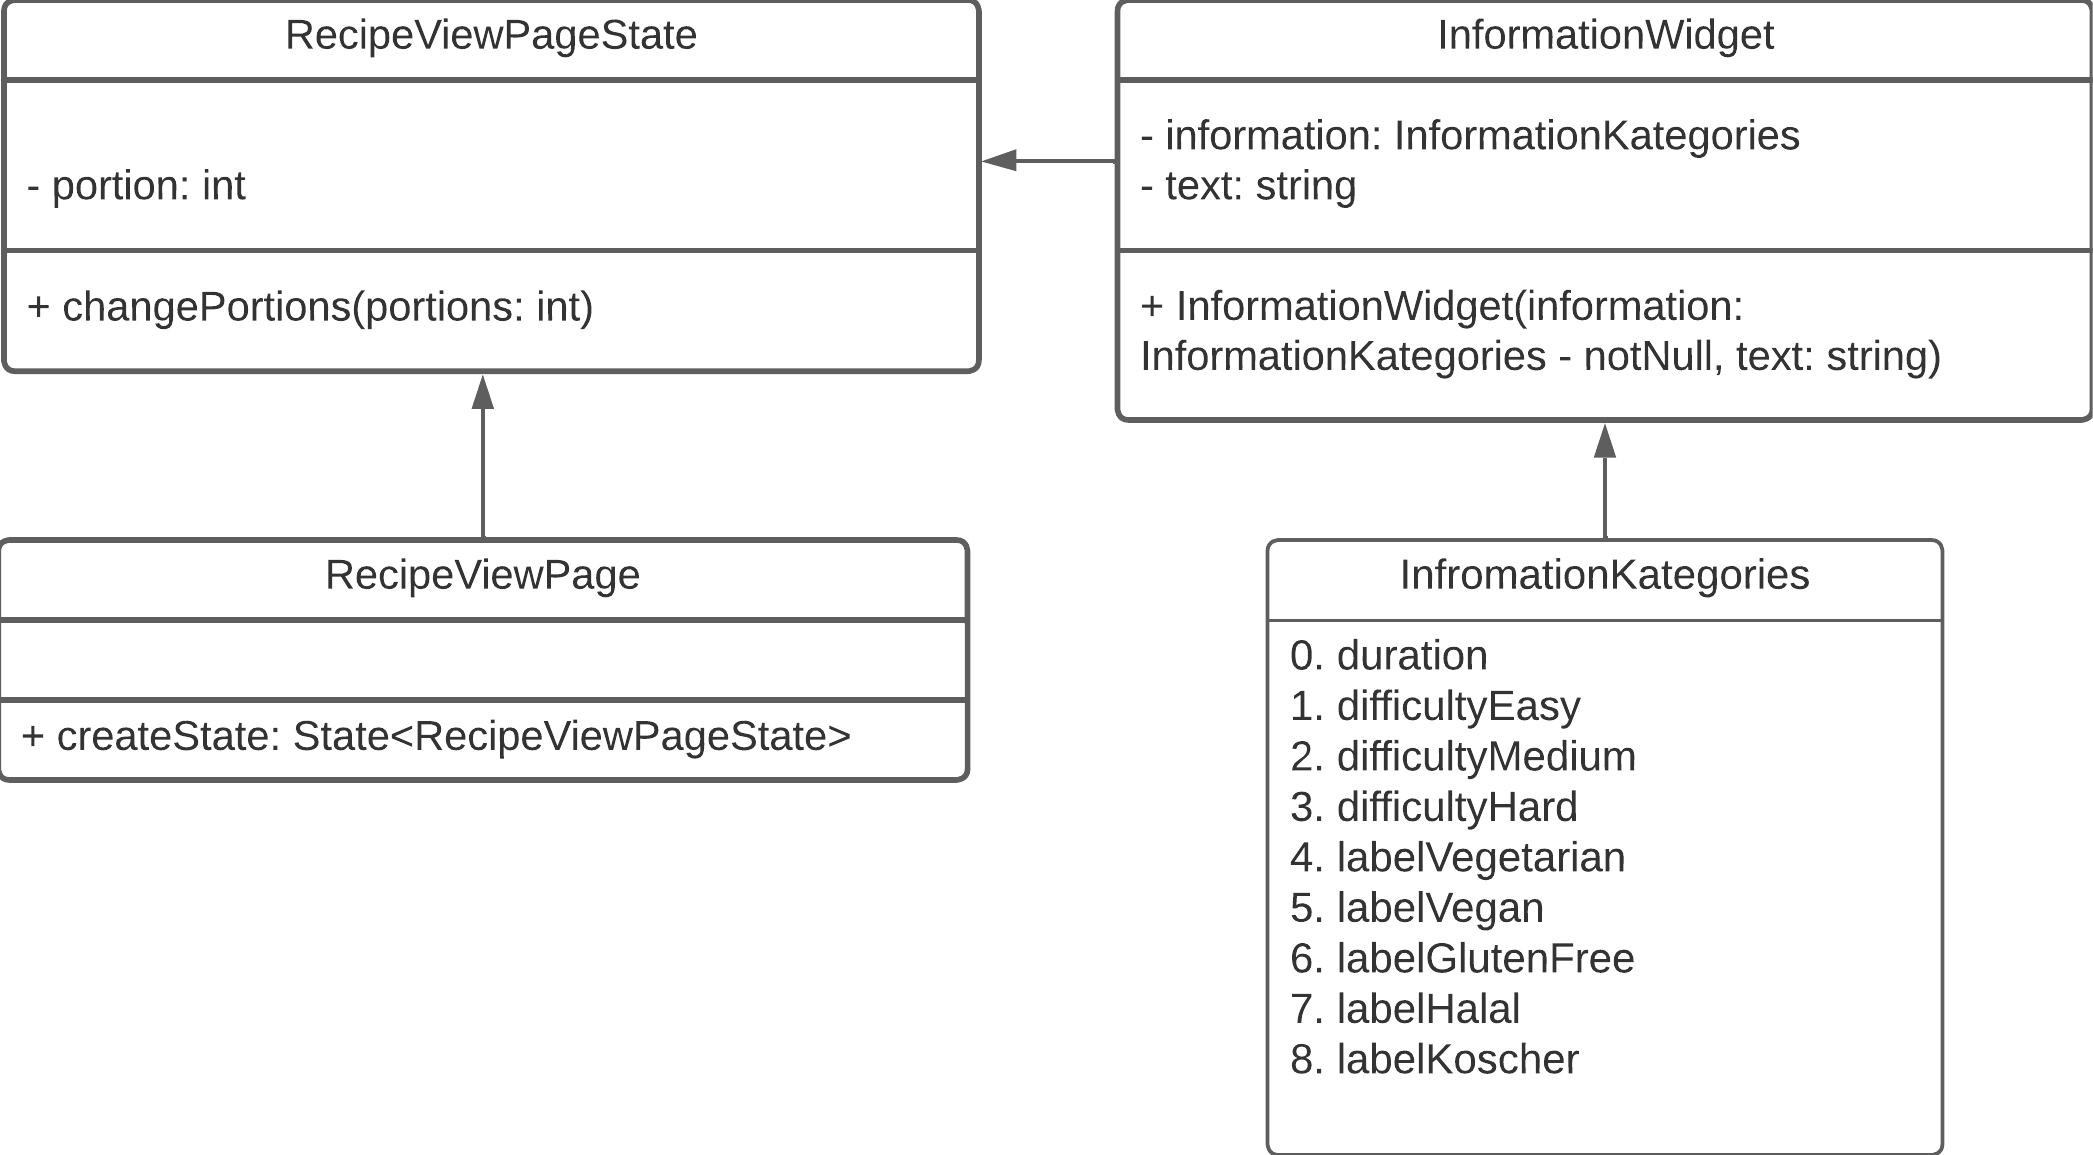
\includegraphics[width=0.95\textwidth]{images/Presentation-layer/RecipeViewClass.png}
            \caption{Klassen für Rezeptansicht}
        \end{minipage}
    \end{figure}    

    \newpage

\subsection{Registrierungsansicht}
    Die Klassen beinhalten alle nötigen Funktionen und Attribute um die Registrierungsansicht darzustellen.

    \subsubsection{RegisterPage}
        \paragraph*{Methode}
            \subparagraph*{createState: State<RegisterPageState>} - Konstruktor für den RegisterPageState.
    
    \subsubsection{RegisterPageState}
        \paragraph*{Attribute}
            \subparagraph*{usernameController: TextEdittingController} - Die eingegebene Zeichenkette für den Benutzernamen des neuen Users.
            \subparagraph*{emailController: TextEdittingController} - Die eingegebene Zeichenkette für die E-Mail-Adresse des neuen Users.
            \subparagraph*{passwordController: TextEdittingController} - Die eingegebene Zeichenkette für das Passwort des neuen Accounts für den neunen User.
            \subparagraph*{repeatedPassword: TextEdittingController} - Die eingegebene Zeichenkette für das wiederholte Passwort des neuen Accounts.
         
        \paragraph*{Methoden}
            \subparagraph*{register(username: string, email: string, password: string, repeatedPassword: string)} - Überprüft ob das eingegeben Passwort mit dem wiederholten Passwort übereinstimmt und ruft dann die Funktion register() im UserRepository auf.
            \subparagraph*{login()} - Die Loginansicht wird aufgerufen.

    \subsubsection{InformationWidget (\autoref{sec:InformationWidget})}

    \subsubsection{InformationKategories (\autoref{sec:InformationKategories})}
    \begin{figure}[htp]
        \begin{minipage}
            [t]{0.49\textwidth}
            \centering
            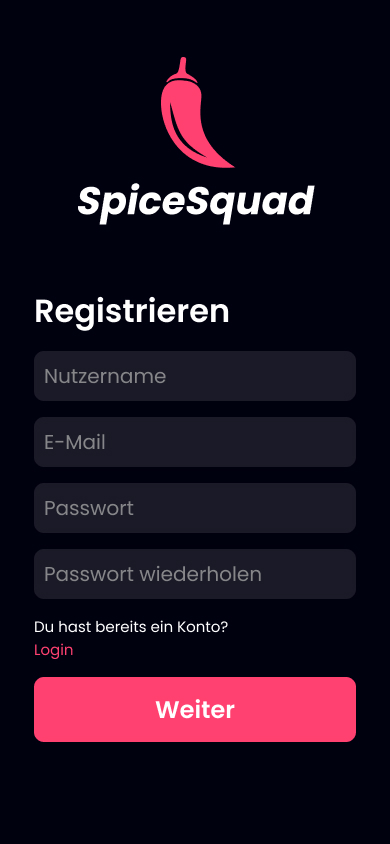
\includegraphics[height=80mm]{images/Presentation-layer/RegisterView.jpg}
            \caption{Registrierungsansicht}
        \end{minipage}
        \begin{minipage}
            [t]{0.49\textwidth}
            \centering
            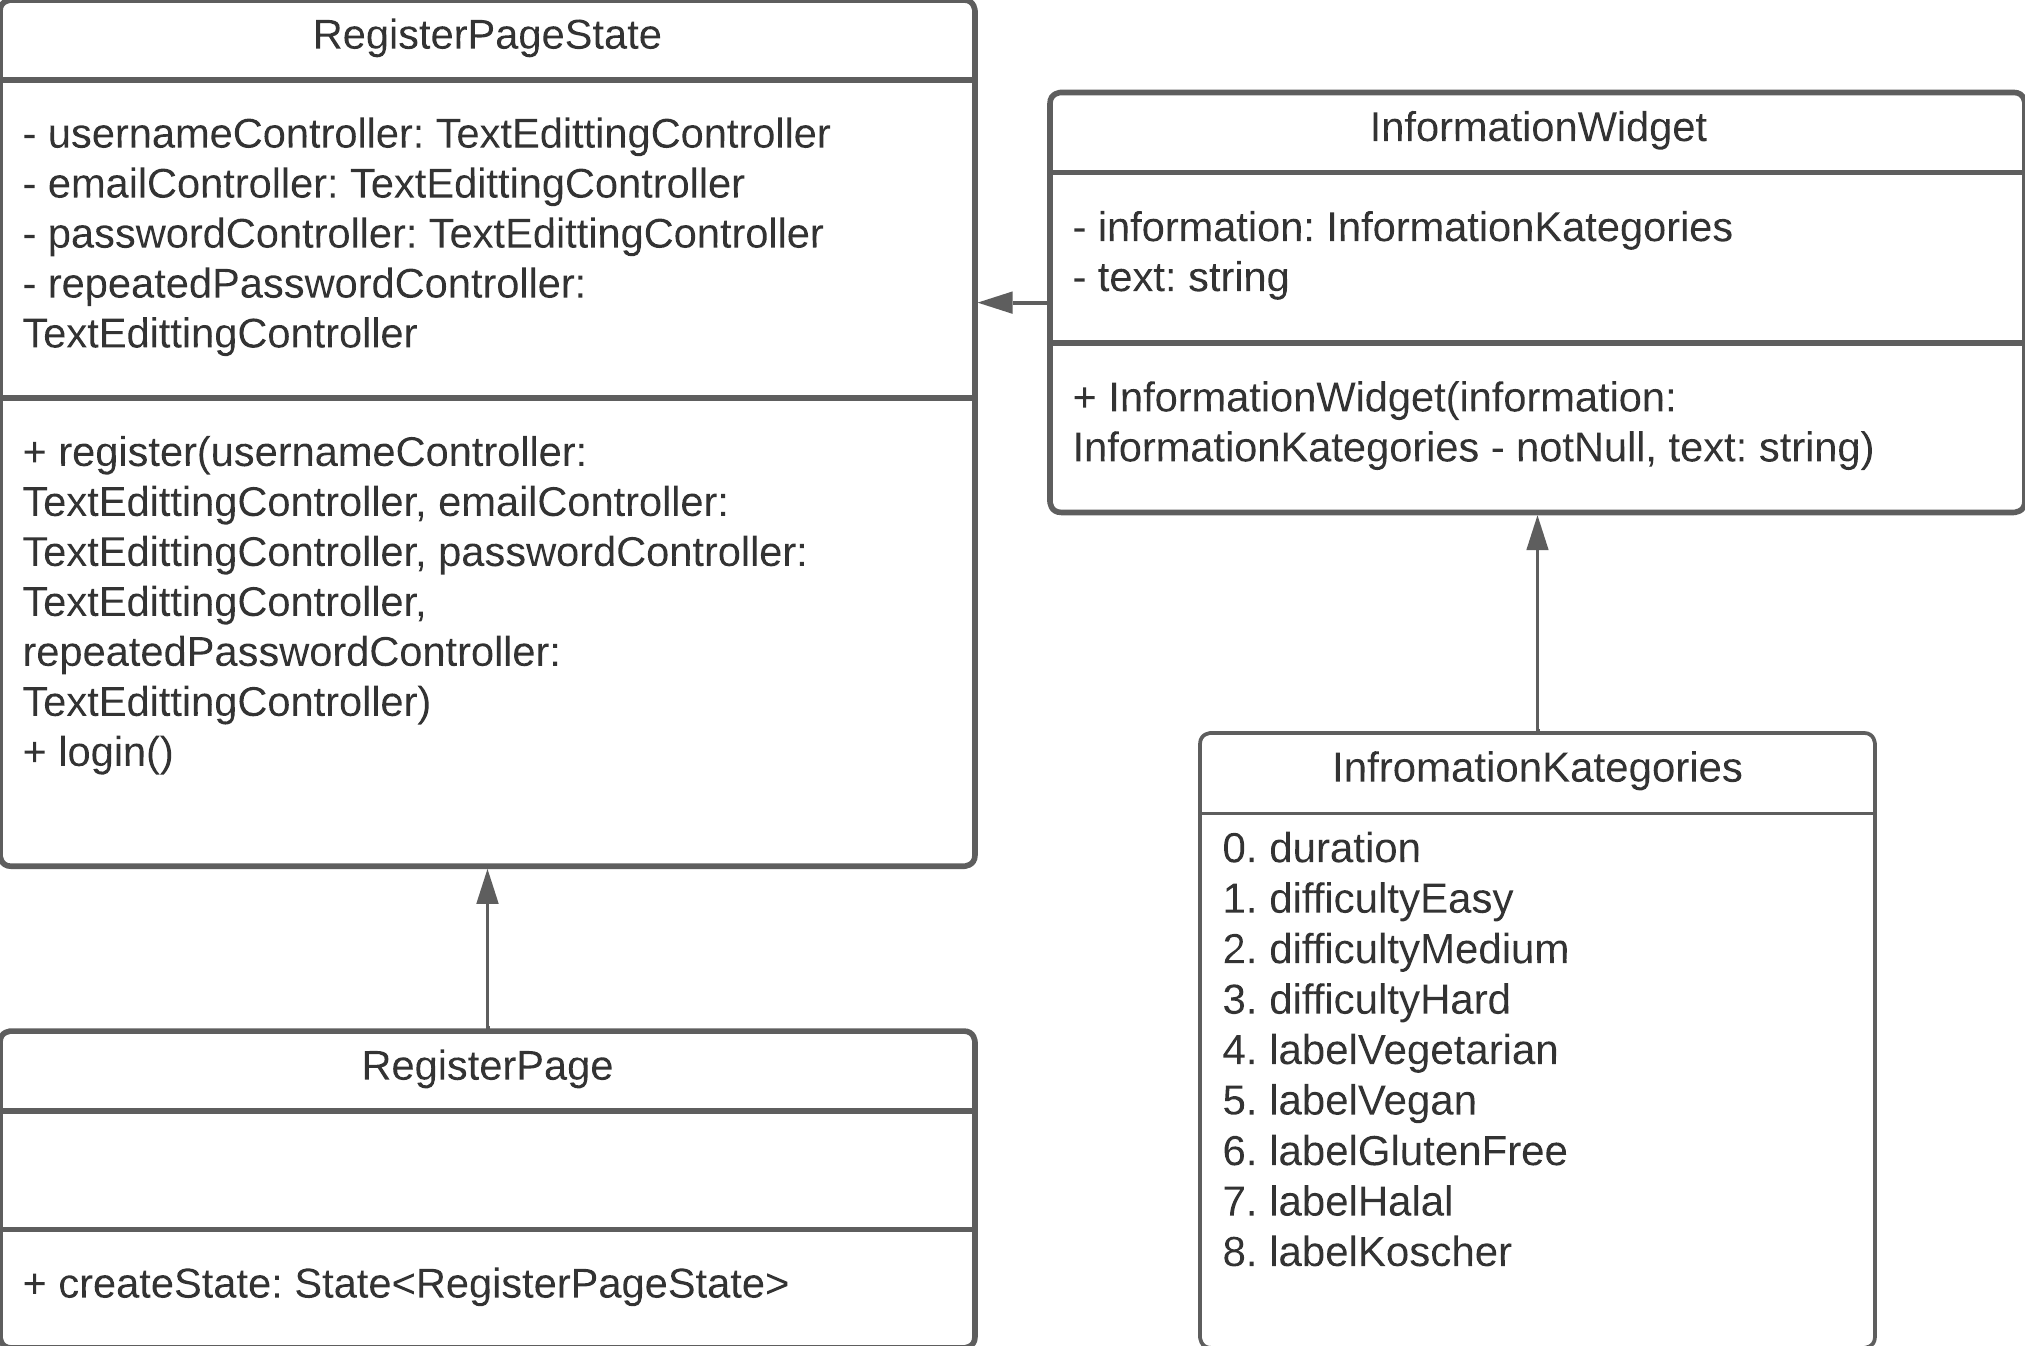
\includegraphics[width=0.95\textwidth]{images/Presentation-layer/RegisterViewClass.png}
            \caption{Klassen für Registrierungsansicht}
        \end{minipage}
    \end{figure}    
        
    \newpage

\subsection{Passwort-Zurücksetzen-Ansicht}
    Die Klassen beinhalten alle nötigen Funktionen und Attribute um die Passwort-Zurücksetzen-Ansicht darzustellen.
    
    \subsubsection{ResetPasswordPage}
        \paragraph*{Methode}
            \subparagraph*{createState: State<ResetPasswordPageState>} - Konstruktor für den ResetPasswordPageState.
    
    \subsubsection{ResetPasswordPageState}
        \paragraph*{Attribut}
            \subparagraph*{emailController: TextEdittingController} - Die eingegebene Zeichenkette für die E-Mail-Adresse des Users.
    
        \paragraph*{Methoden}
            \subparagraph*{resetPassword(email: string)} - Überprüft ob die Korrektheit der E-Mail-Adresse und ruft die Funktionen resetPassword() im UserRepository auf.
            \subparagraph*{LoginView()} - Die Loginansicht wird aufgerufen.

    \subsubsection{ReturnButton} \label{sec:ReturnButton}
        \paragraph*{Methoden}
            \subparagraph*{prevoiusView()} - Die vorherige Ansicht wird aufgerufen. Es werden keine Daten gespeichert die in der Ansicht angegeben worden sind.
    
            \begin{figure}[htp]
                \begin{minipage}
                    [t]{0.49\textwidth}
                    \centering
                    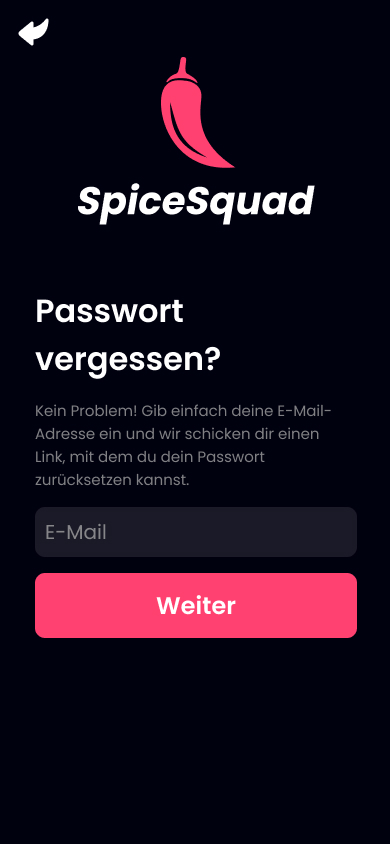
\includegraphics[height=80mm]{images/Presentation-layer/PasswordResetView.jpg}
                    \caption{Passwort-Zurücksetzen-Ansicht}
                \end{minipage}
                \begin{minipage}
                    [t]{0.49\textwidth}
                    \centering
                    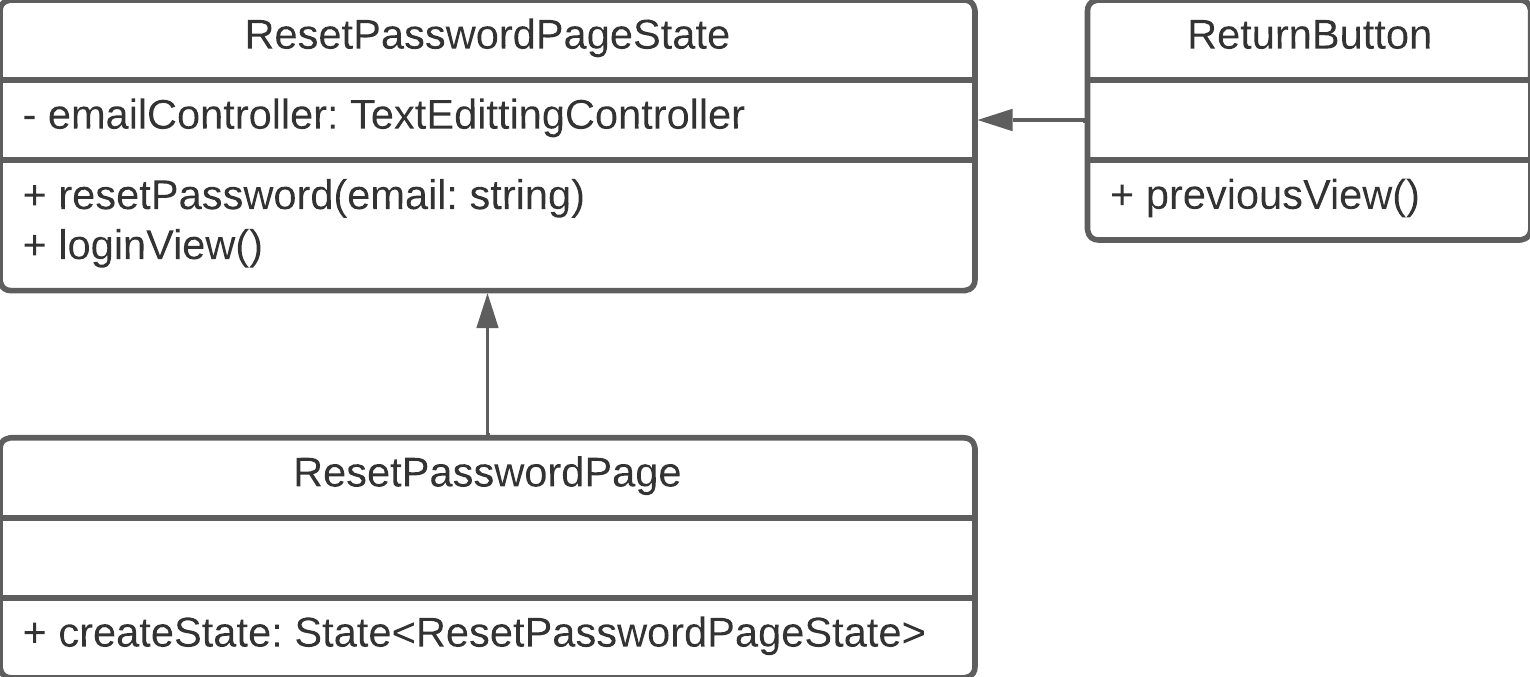
\includegraphics[width=0.95\textwidth]{images/Presentation-layer/PasswordResetViewClass.png}
                    \caption{Klassen für Passwort-Zurücksetzen-Ansicht}
                \end{minipage}
            \end{figure}    
        
            \newpage

\subsection{Anmeldungsansicht}
    Die Klassen beinhalten alle nötigen Funktionen und Attribute um die Anmeldungsansicht darzustellen.

    \subsubsection{LoginPagePage}
        \paragraph*{Methode}
            \subparagraph*{createState: State<LoginPageState>} - Konstruktor für den LoginPageState.
    
    \subsubsection{LoginPageState}
        \paragraph*{Attribut}
            \subparagraph*{emailController: TextEdittingController} - Die eingegebene Zeichenkette für die E-Mail-Adresse des Users.
            \subparagraph*{passwortController: TextEdittingController} - Die eingegebene Zeichenkette für das Passwort des Users.

        \paragraph*{Methoden}

            \subparagraph*{login(email: string, password: string)} - Überprüft die Eingaben und ruft die Funktionen createGroupe() im UserRepository auf.
            \subparagraph*{resetPasswordView()} -  Die Passwort-Zurücksetzen-Ansicht wird aufgerufen.
            \subparagraph*{registerView()} -  Die Registrierungsansicht wird aufgerufen.

    \begin{figure}[htp]
        \begin{minipage}
            [t]{0.49\textwidth}
            \centering
            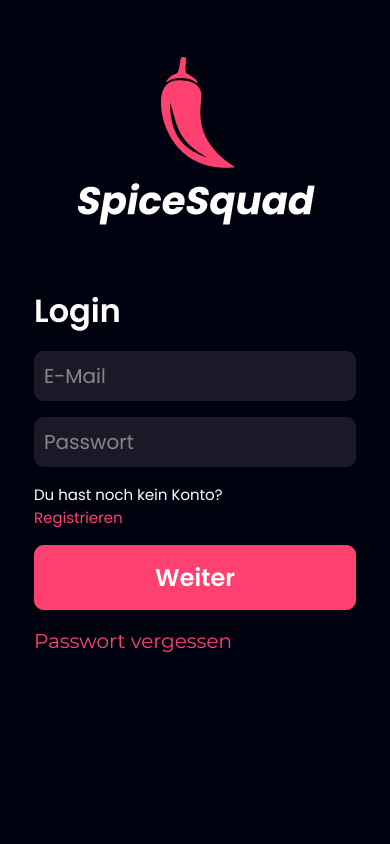
\includegraphics[height=80mm]{images/Presentation-layer/LoginView.jpg}
            \caption{Anmeldungsansicht}
        \end{minipage}
        \begin{minipage}
            [t]{0.49\textwidth}
            \centering
            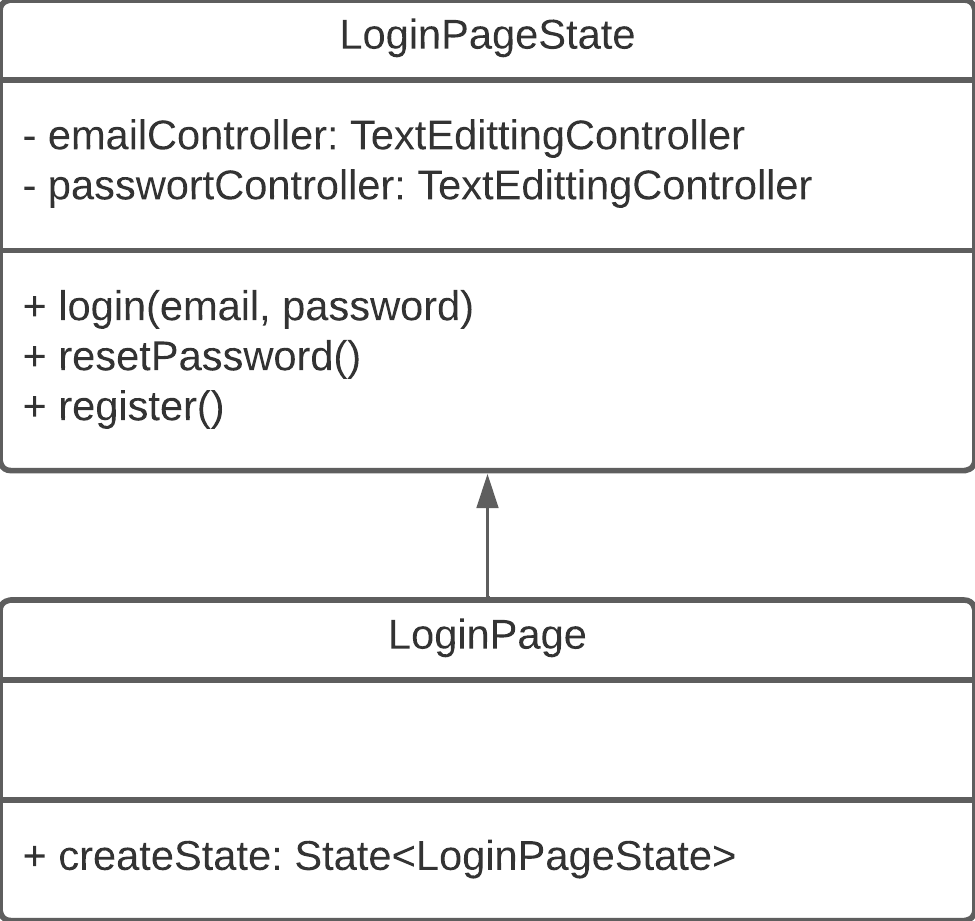
\includegraphics[width=0.95\textwidth]{images/Presentation-layer/LoginViewClass.png}
            \caption{Klassen für Anmeldungsansicht}
        \end{minipage}
    \end{figure}    
        
    \newpage

\subsection{Gruppen-Erstellungs-Ansicht}
    Die Klassen beinhalten alle nötigen Funktionen und Attribute um die Gruppen-Erstellungs-Ansicht darzustellen.

    \subsubsection{GroupeCreationPage}
        \paragraph*{Methode}
            \subparagraph*{createState: State<GroupeCreationPageState>} - Konstruktor für den GroupeCreationPageState.
    
    \subsubsection{GroupeCreationPageState}
        \paragraph*{Attribut}
            \subparagraph*{groupeNameController: TextEdittingController} - Die eingegebene Zeichenkette für den Namen der neuen Gruppe.

        \paragraph*{Methoden}

            \subparagraph*{createGroupe(name: string)} - Überprüft den Gruppenname und ruft die Funktionen createGroupe() im GroupeService auf.
            \subparagraph*{joinGroupeView()} -  Die Gruppen-Beitritts-Ansicht wird aufgerufen.
    \begin{figure}[htp]
        \begin{minipage}
            [t]{0.49\textwidth}
            \centering
            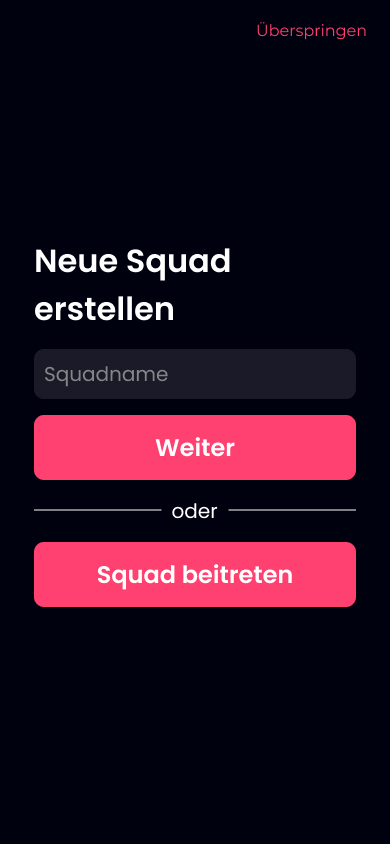
\includegraphics[height=80mm]{images/Presentation-layer/GroupCreationView.jpg}
            \caption{Passwort-Zurücksetzen-Ansicht}
        \end{minipage}
        \begin{minipage}
            [t]{0.49\textwidth}
            \centering
            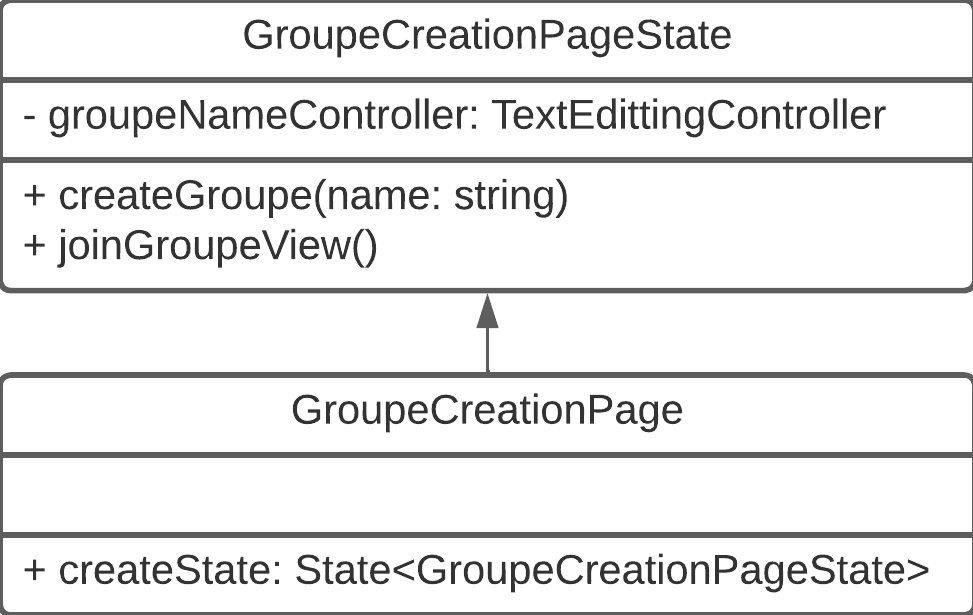
\includegraphics[width=0.95\textwidth]{images/Presentation-layer/GroupCreationViewClass.png}
            \caption{Klassen für Passwort-Zurücksetzen-Ansicht}
        \end{minipage}
    \end{figure}    
        
    \newpage

\subsection{Gruppen-Detail-Ansicht}
    Die Klassen beinhalten alle nötigen Funktionen und Attribute um die Gruppen-Detail-Ansicht darzustellen.

    \subsubsection{GroupDetailPage}
        \paragraph*{Attribut}
            \subparagraph*{group: Group} - Die Gruppe dessen Details dargestellt werden.
            \subparagraph*{newTitle: TextEdittingController} - Die eingegeben Zeichenkette für den neunen Gruppennamen.

        \paragraph*{Methoden}
            \subparagraph*{GroupDetailPage(group: Group - notNull)} - Ein Konstruktor für eine GroupDetailPage. Der Parameter muss angegeben werden. 
            \subparagraph*{setGroupTitle(newTitle: string)} - Die Eingabe wird Überprüft und die Funktion setGroupName() im GroupeService wird aufgerufen.
            \subparagraph*{deleteGroup()} - Das ConfirmationWidget wird aufgerufen und bei positiver Rückmeldung wird die Funktion kickUser() im GroupeService wird aufgerufen. Bei negativer Rückmeldung ändert sich nichts.
            \subparagraph*{leaveGroup()} - Das ConfirmationWidget wird aufgerufen und bei positiver Rückmeldung wird die Funktion leaveGroup() im GroupeService wird aufgerufen. Bei negativer Rückmeldung ändert sich nichts.
            \subparagraph*{getQRCode()} - Die QR-Code-Ansicht wird aufgerufen.
            \subparagraph*{getGroupeTitel()} - Der Gruppen Titel wird in die Zwischenablage gespeichert.

    \subsubsection{ConfirmationWidget}
        \paragraph*{Attribut}
            \subparagraph*{text: string} - Der Text der Angezeigt werden soll im Widget.

        \paragraph*{Methoden}
            \subparagraph*{ConfirmationWidget(text: string - notNull)} - Ein Konstruktor für ein ConfirmationWidget, wobei ein Text angegeben werden muss.
            \subparagraph*{decline()} - Dem Erzeugter wird true zurückgegeben.
            \subparagraph*{accept()} - Dem Erzeugter wird false zurückgegeben.

    \subsubsection{OptionWidget}
        \paragraph*{Attribut}
            \subparagraph*{user: User} - Der darzustellende User.

        \paragraph*{Methoden}
            \subparagraph*{OptionWidget(user: User - notNull)} - Ein Konstruktor für ein OptionWidget. Der Parameter muss angegeben werden. 
            \subparagraph*{kickUser()} - Das ConfirmationWidget wird aufgerufen und bei positiver Rückmeldung wird die Funktion kickUser() im UserSettingsService wird aufgerufen. Bei negativer Rückmeldung ändert sich nichts.
            \subparagraph*{banUser()} - Das ConfirmationWidget wird aufgerufen und bei positiver Rückmeldung wird die Funktion banUser() im UserSettingsService wird aufgerufen. Bei negativer Rückmeldung ändert sich nichts.
            \subparagraph*{makeAdmin()} - Das ConfirmationWidget wird aufgerufen und bei positiver Rückmeldung wird die Funktion makeAdmin() im UserSettingsService wird aufgerufen. Bei negativer Rückmeldung ändert sich nichts.
            \subparagraph*{removeAdminStatus()} - Das ConfirmationWidget wird aufgerufen und bei positiver Rückmeldung wird die Funktion removeAdminStatus() im UserSettingsService wird aufgerufen. Bei negativer Rückmeldung ändert sich nichts.

    \subsubsection{RecipeWidget}
        \paragraph*{Attribut}
            \subparagraph*{recipe: Recipe} - Das darzustellende Rezept.
            \subparagraph*{view: Boolean} - Ein Boolean der Angibt ob die Sichtbarkeit des Rezepts verändert werden darf oder nicht.
            \subparagraph*{settingsView: Boolean} - Eine Boolean der angibt ob das Widget in der Einstellungsansicht verwendet wird.

        \paragraph*{Methoden}
            \subparagraph*{RecipeWidget(recipe: Recipe - notNull, view: boolean - notNull, settingsView: boolean - notNull)} - Ein Konstruktor für ein RecipeWidget. Alle Parameter müssen angegeben werden.
            \subparagraph*{togglePrivate()} - Die Sichtbarkeit des Rezepts für die Gruppe ausgeblendet werden soll, wenn settingsView false ist. Wenn settingsView auf true steht wird das Rezept für alle Gruppen ausgeblendet.
            \subparagraph*{delete()} - Das ConfirmationWidget wird aufgerufen und bei positiver Rückmeldung wird die Funktion deleteRecipe() im RecipeService aufgerufen. Bei negativer Rückmeldung ändert sich nichts.
            \subparagraph*{export()} - Die Funktion exportRecipe() im RecipeService wird aufgerufen.

    \subsubsection{UserWidget}
        \paragraph*{Attribut}
            \subparagraph*{isOwnAccount: Boolean} - Ein Boolean der Angibt ob es sich um den eigenen Account handelt.

        \paragraph*{Methoden}
            \subparagraph*{UserWidget(user: User - notNull, isOwnAccount: bool - notNull)} - Ein Konstruktor für ein UserWidget. Alle Parameter müssen angegeben werden.
            \subparagraph*{options()} - Das optionWidget wird aufgerufen.

    \subsubsection{ReturnButton (\autoref{sec:ReturnButton})}

    \begin{figure}[htp]
        \begin{minipage}
            [t]{0.49\textwidth}
            \centering
            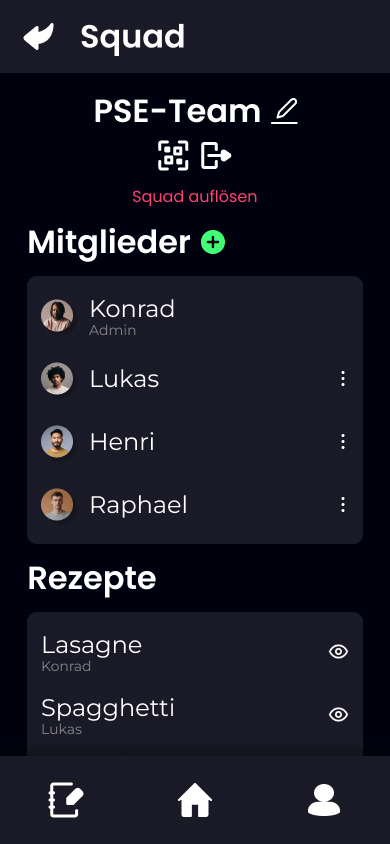
\includegraphics[height=80mm]{images/Presentation-layer/GroupDetailView.jpg}
            \caption{Gruppen-Detail-Ansicht}
        \end{minipage}
        \begin{minipage}
            [t]{0.49\textwidth}
            \centering
            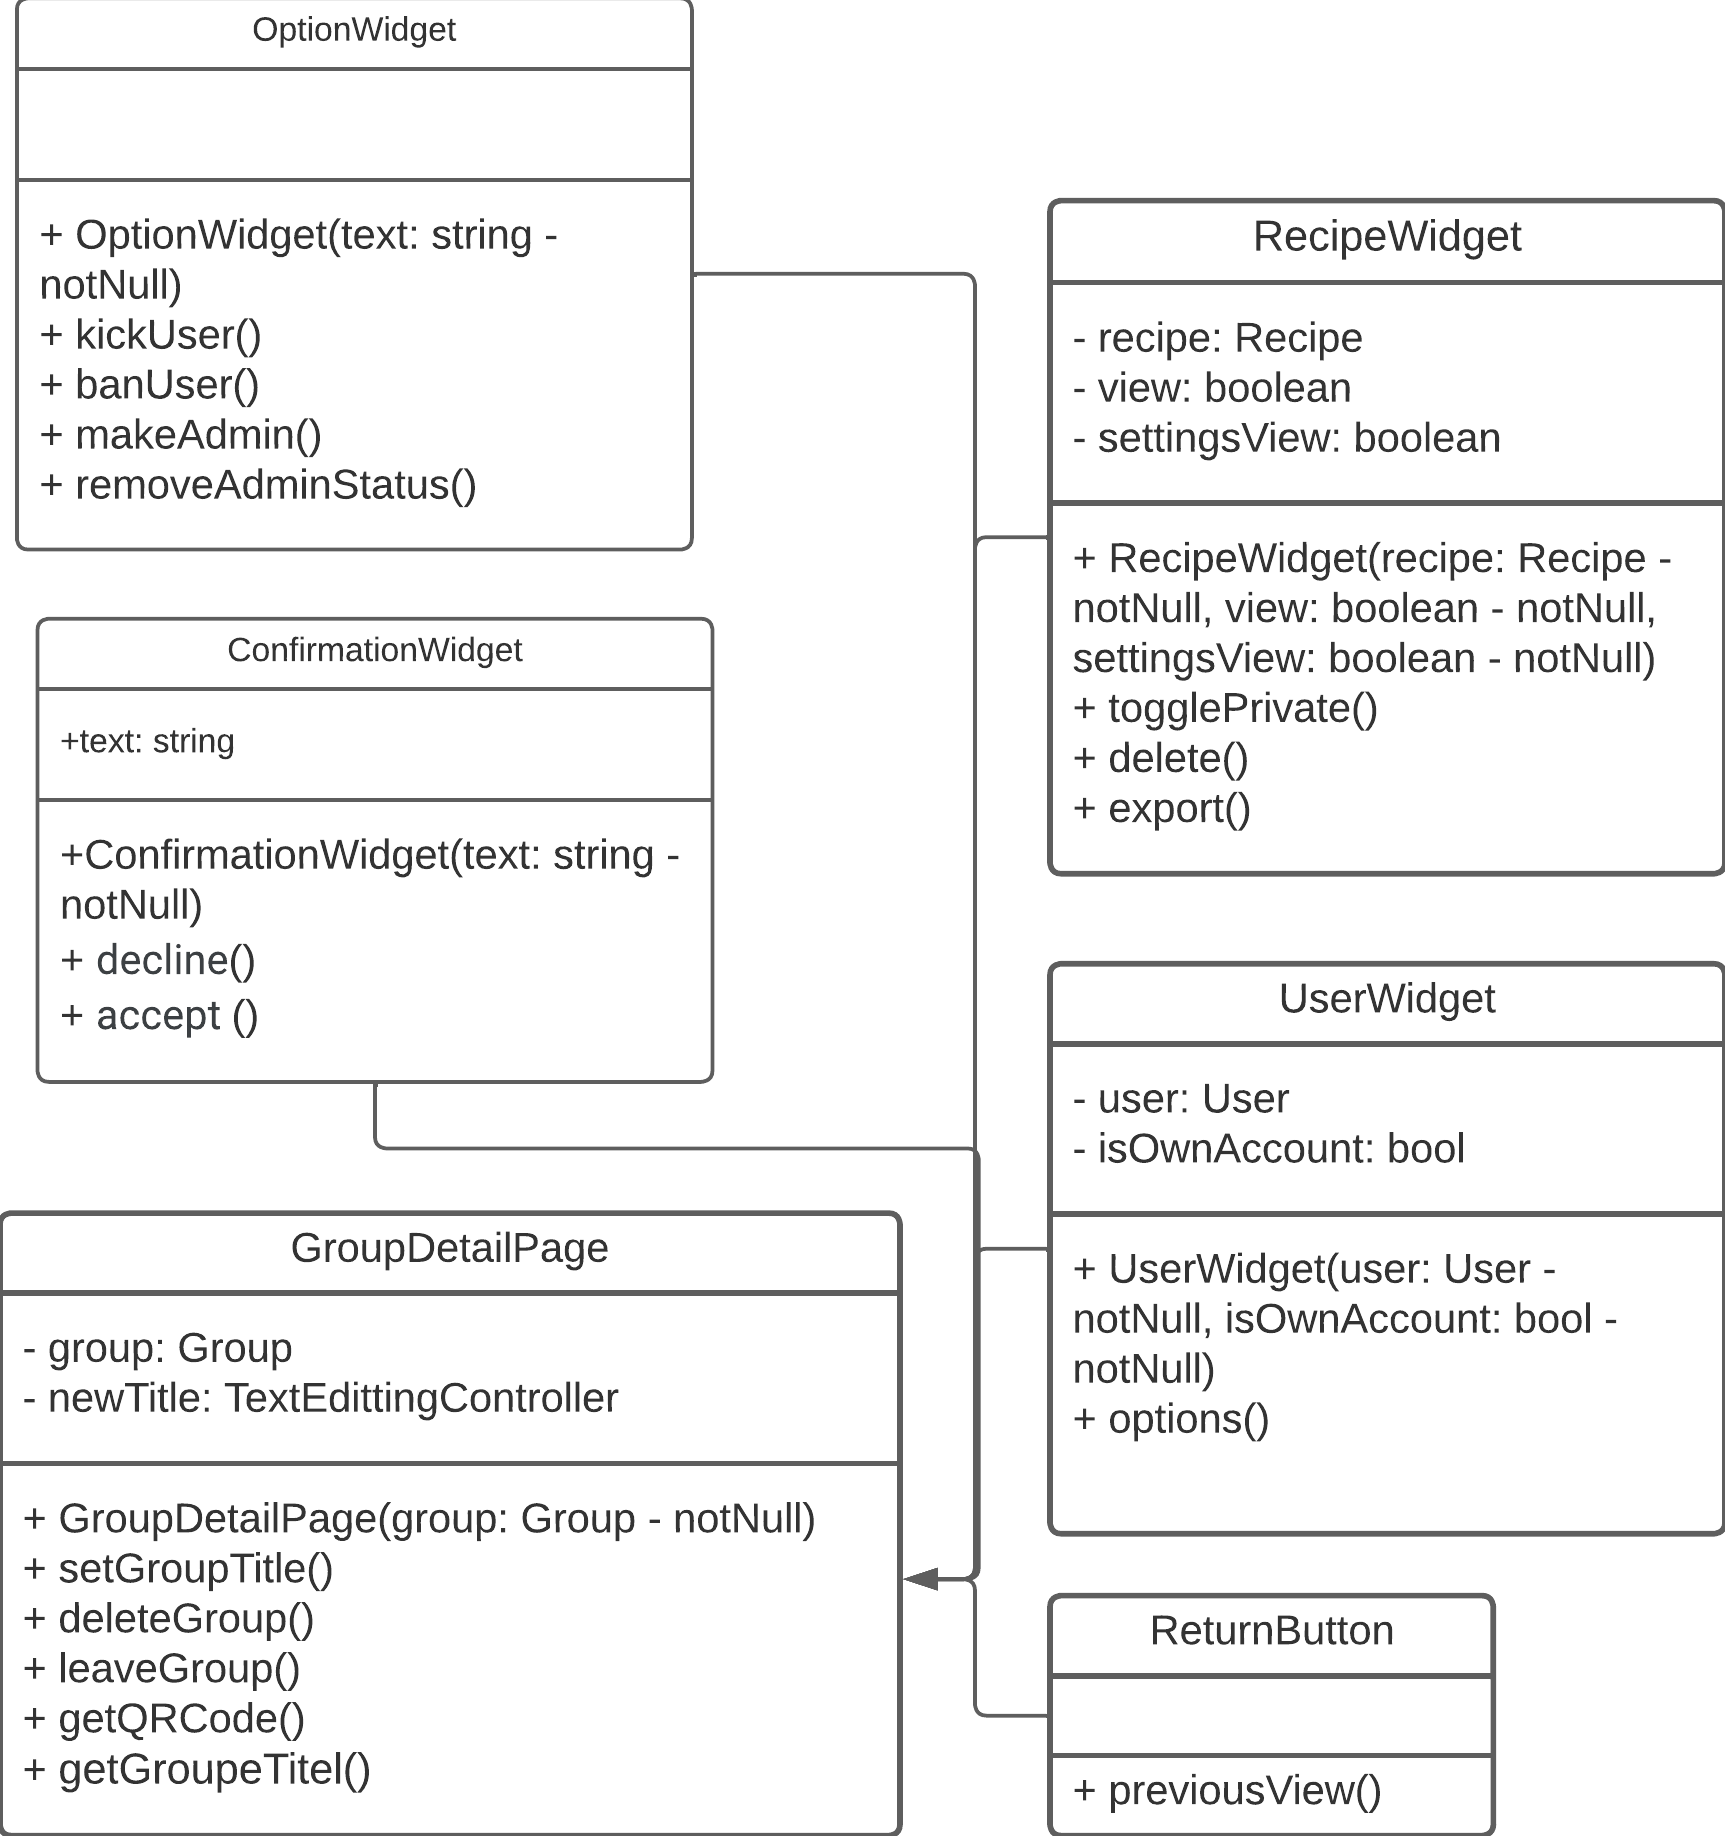
\includegraphics[width=0.95\textwidth]{images/Presentation-layer/GroupDetailViewClass.png}
            \caption{Klassen für Gruppen-Detail-Ansicht}
        \end{minipage}
    \end{figure}    
        
    \newpage
  
  \subsection{Rezept-Erstellungs-Ansicht}
    Die Klassen beinhalten alle nötigen Funktionen und Attribute um die Rezept-Erstell-Ansicht darzustellen.\newline

    \subsubsection{RecipeCreationPageState}
        \paragraph*{Attributes}
            \subparagraph*{image: blob} - Hochgeladenes Bild, welches den anderen Nutzern in der Rezeptansicht angezeigt werden soll.
            \subparagraph*{title: TextEdittingController (notNull)} - Die eingegebene Zeichenkette für den Titel des Rezepts. Die Zeichenkette kann maximal 64 Zeichen lang sein und muss ausgefüllt sein.
            \subparagraph*{is\_Vegetarian: Boolean} - Der vom Nutzer angegebene Boolean, ob das \gls{label} Vegetarisch dem Leser angezeigt werden soll. Ist standartmäßig auf false.
            \subparagraph*{is\_Vegan: Boolean} - Der vom Nutzer angegebene Boolean, ob das \gls{label} Vegan dem Leser angezeigt werden soll. Ist standartmäßig auf false.
            \subparagraph*{is\_GlutenFree: Boolean} - Der vom Nutzer angegebene Boolean, ob das \gls{label} Glutenfrei dem Leser angezeigt werden soll.  Ist standartmäßig auf false.
            \subparagraph*{is\_Halal: Boolean} - Der vom Nutzer angegebene Boolean, ob das \gls{label} Halal dem Leser angezeigt werden soll.  Ist standartmäßig auf false.
            \subparagraph*{is\_Kosher: Boolean} - Der vom Nutzer angegebene Boolean, ob das \gls{label} Koscher dem Leser angezeigt werden soll.  Ist standartmäßig auf false.
            \subparagraph*{duration: TextEdittingController (notNull)} - Die vom Nutzer eingegebene Ganzzahl, welche die Zubereitungszeit in Minuten angibt. Muss angegeben werden.
            \subparagraph*{difficulty: Difficulty (notNull)} - Die vom Nutzer ausgewählte \gls{schwierigkeit} des Rezepts. Muss angegeben werden.
            \subparagraph*{ingredients: Ingredients[]} - Eine Liste an Ingerdients, welche in der AddIngredientPage erstellt wurde.
            \subparagraph*{instructions: TextEdittingController (notNull)} - Die vom Nutzer angegeben Zeichenkette für die Beschreibung des Rezepts. Muss angegeben werden.

        \paragraph*{Methods}
            \subparagraph*{addIngredient()} - Die Page AddIngredientPage wird aufgerufen.
            \subparagraph*{recipeSave()} - Die Methode ruft, abhängig davon ob das Rezept neu erstellt wird oder nur verändert wurde, entweder recipeCreation() oder recipeChange() auf.
       
            
        \begin{figure}[htp]
            \begin{minipage}
                [t]{0.49\textwidth}
                \centering
                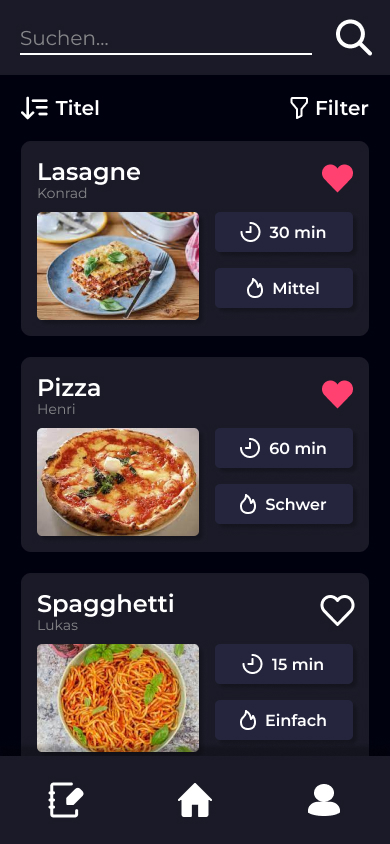
\includegraphics[height=80mm]{images/Presentation-layer/MainView.jpg}
                \caption{Hauptansicht}
            \end{minipage}
            \begin{minipage}
                [t]{0.49\textwidth}
                \centering
                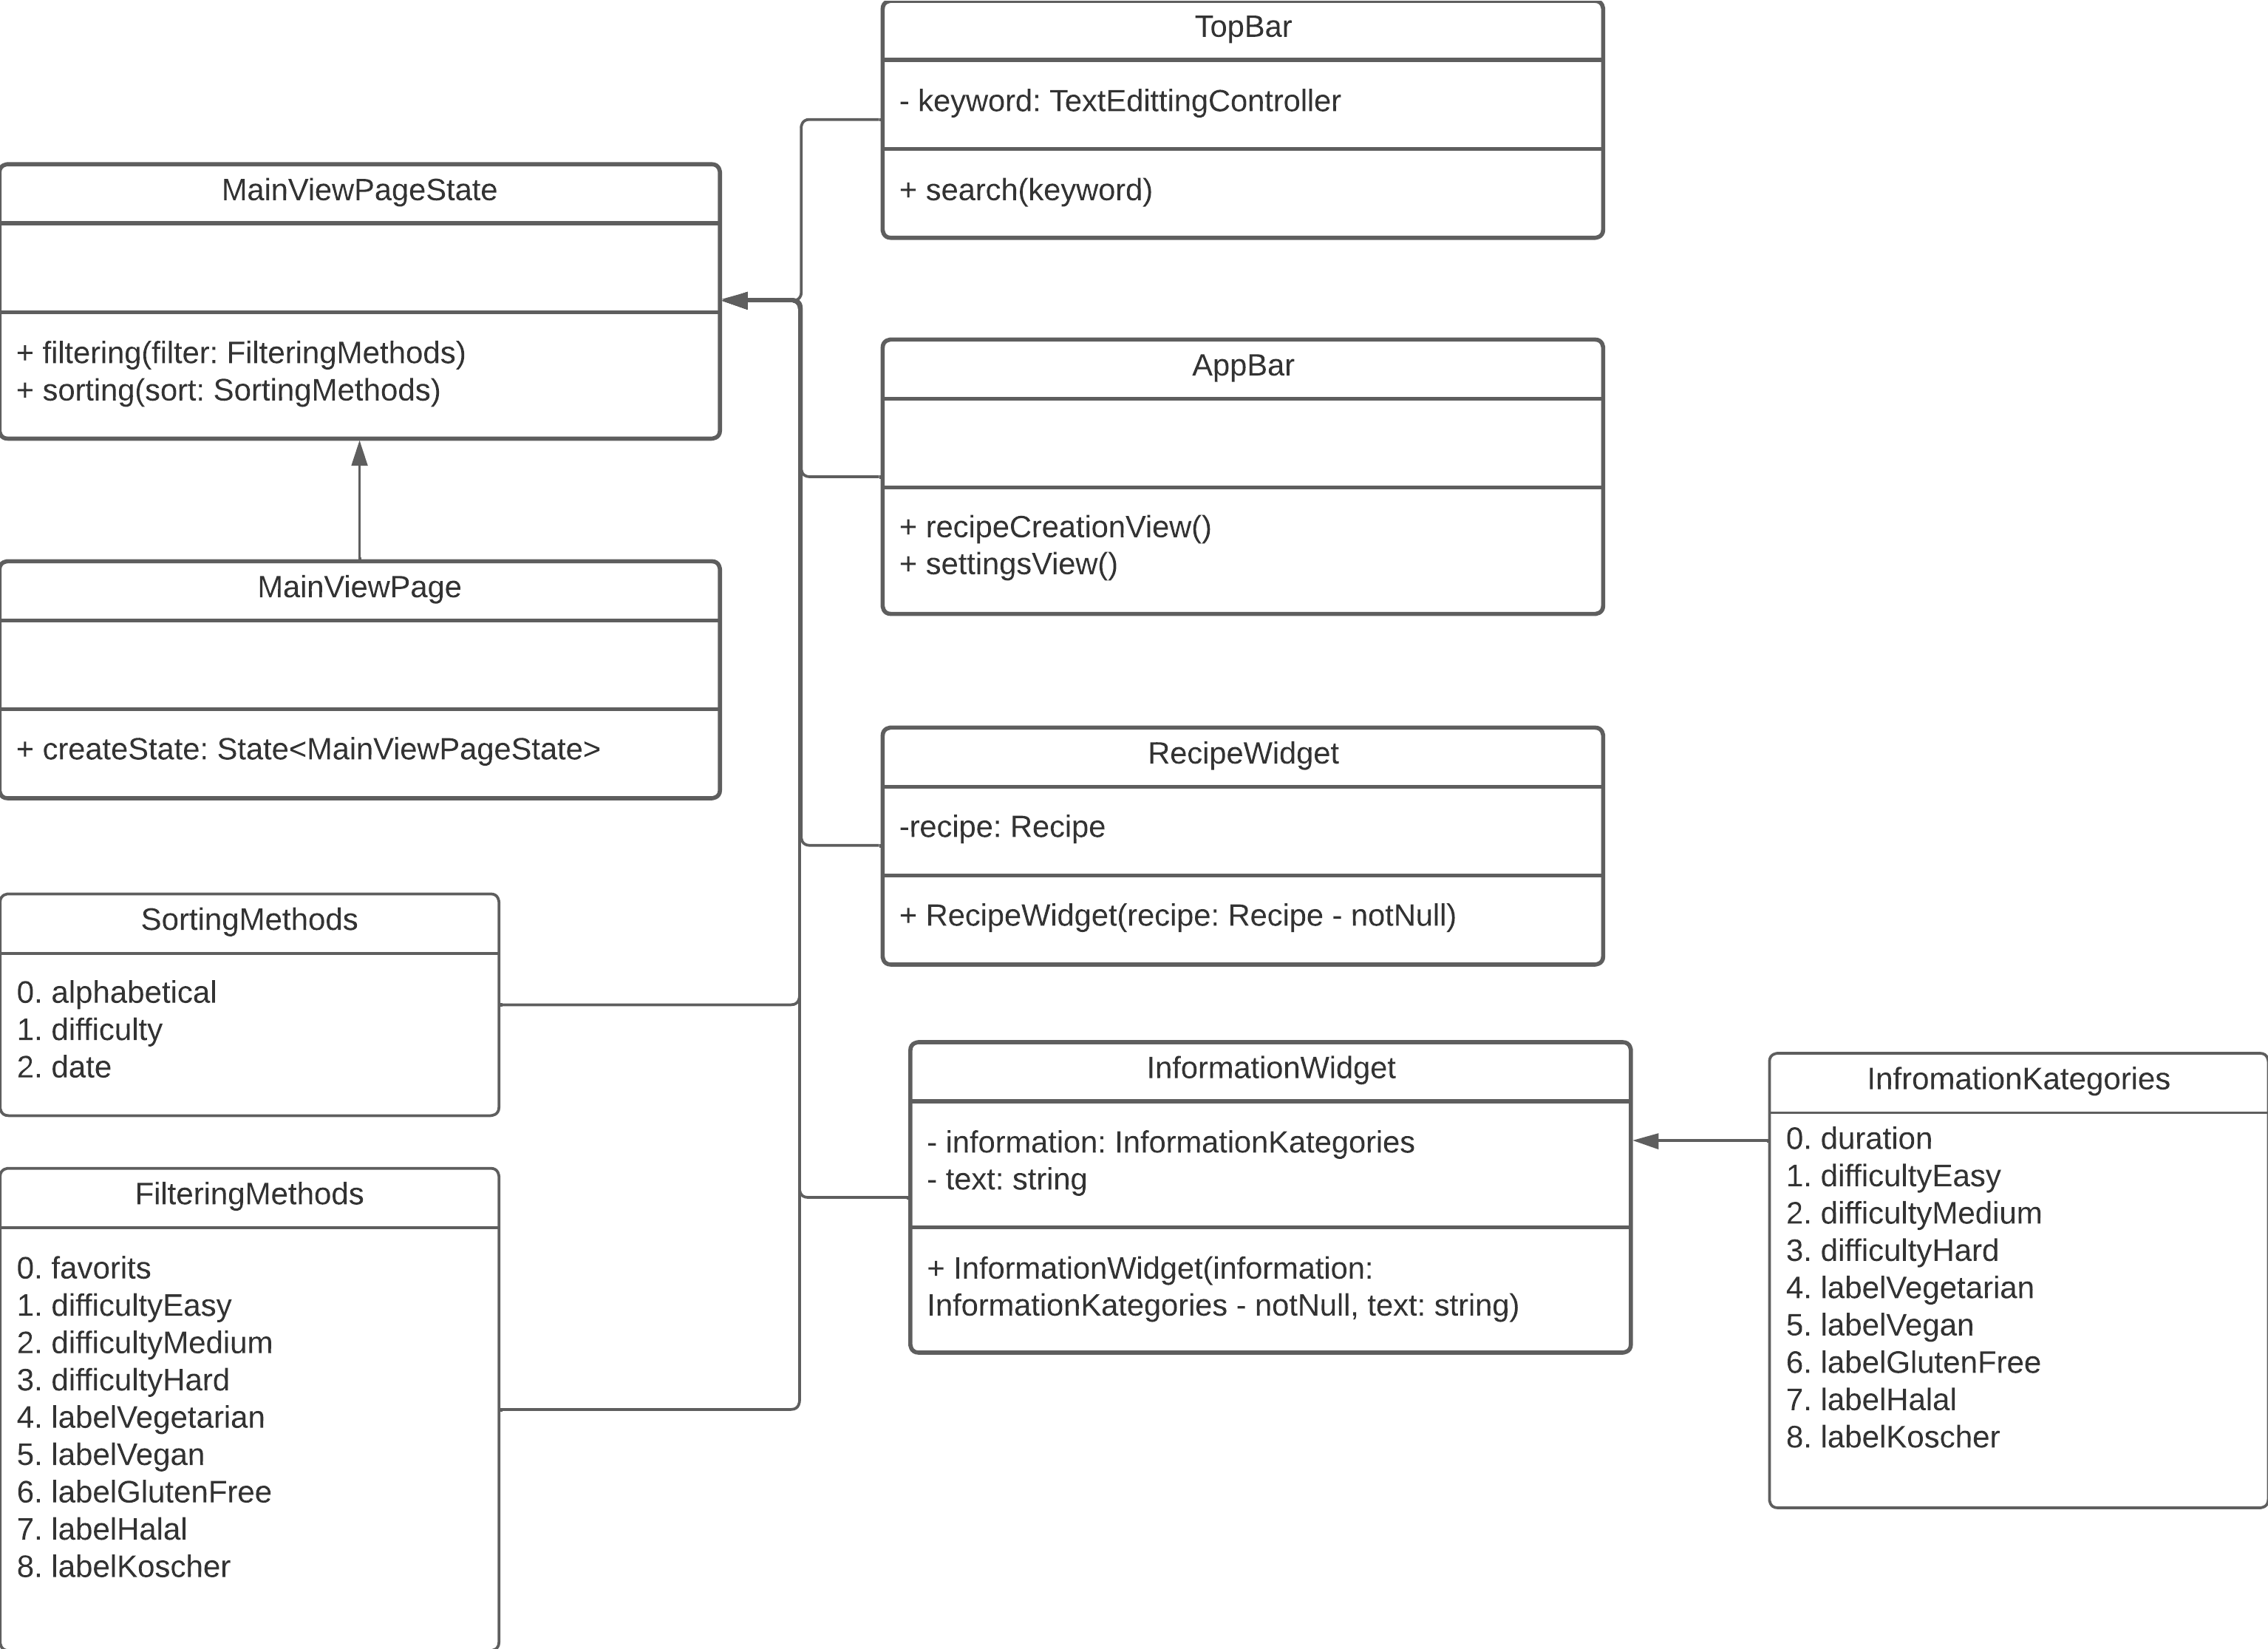
\includegraphics[width=0.95\textwidth]{images/Presentation-layer/MainViewClass.png}
                \caption{Klassen für Hauptansicht}
            \end{minipage}
        \end{figure}
    \newpage

\newpage

\section{REST-Webservice}

\subsection{Server}
\subsection*{Attribute}
\paragraph{port: number} Durch das Attribut port lässt sich einstellen auf welchen Port Anfragen an den Server zulässig sind.
Port ist vom Type number.
\paragraph{firebaseCredentials: any}
\paragraph{express: express.Application}
\paragraph{app: App}
\paragraph{}

\subsection*{Methode}
\paragraph{public <<create>> constructor(): void}
\paragraph{public start(): void}
\paragraph{private connectToDatabase(): void}
\paragraph{private connectToFirebase(): void}
\paragraph{private createServer(): void}


\subsection{App}
\subsubsection*{Attribute}
\paragraph{app: express.Application}
\paragraph{authentificationRoutes: AuthentificationRouter}
\paragraph{recipeRoutes: RecipeRouter}
\paragraph{groupRoutes: GroupRouter}
\paragraph{userRoutes: UserRouter}
\paragraph{IngredientRouter}

\subsubsection*{Methode}
\paragraph{public <<create> constructor(express.Application): void}
\paragraph{private initializeMiddleware(): void}
\paragraph{private initializeRoutes(): void}
\paragraph{privtate initializeErrorHandlers(): void}

\subsection{Router}
\subsubsection{AbstractRouter}
\subsubsection*{Attribute}
\paragraph{protected router: express.Router}
\paragraph{protected controller: AbstractController}
\paragraph{protected checkAuthorization: CheckAuthorization}
\paragraph{protected checkAuth: any}

\subsubsection*{Methode}
\paragraph{public <<create>> constructor(): void}
\paragraph{protected abstract setupRoutes(): void}
\paragraph{public getRouter(): express.Router}

\subsubsection{AuthentificationRouter}
\subsubsection*{Methode}
\paragraph{public <<create>> constructor(): void}
\paragraph{protected setupRoutes(): void}

\subsubsection{RecipeRouter}
\subsubsection*{Methode}
\paragraph{public <<create>> constructor(): void}
\paragraph{protected setupRoutes(): void}

\subsubsection{GroupRouter}
\subsubsection*{Methode}
\paragraph{public <<create>> constructor(): void}
\paragraph{protected setupRoutes(): void}

\subsubsection{UserRouter}
\subsubsection*{Methode}
\paragraph{public <<create>> constructor(): void}
\paragraph{protected setupRoutes(): void}

\subsubsection{IngredientRouter}
\subsubsection*{Methode}
\paragraph{public <<create>> constructor(): void}
\paragraph{protected setupRoutes(): void}

\subsection{Middleware}
\subsubsection{CheckAuthorization}
\subsubsection*{Methode}
\paragraph{authChecker(req: any, res, any, next: any): void}

\subsection{Controller}
\subsubsection{AbstractController}
\subsubsection*{Methode}


\subsubsection{AuthentificationController}
\subsubsection*{Methode}
\paragraph{public userRegister(req: any, res: any, next: any): void}
\paragraph{public userLogin(req: any, res: any, next: any): void}
\paragraph{userResetPassword(req: any, res: any, next: any): void}
\paragraph{}

\subsubsection{RecipeController}
\subsubsection*{Methode}
\paragraph{public recipePost(req: any, res: any, next: any): void}
\paragraph{public recipeDelete(req: any, res: any, next: any): void}
\paragraph{public recipePatch(req: any, res: any, next: any): void}
\paragraph{public recipeGet(req: any, res: any, next: any): void}
\paragraph{public recipeGetAll(req: any, res: any, next: any): void}
\paragraph{public recipeSetFavorite(req: any, res: any, next: any): void}
\paragraph{public recipeGetByGroup(req: any, res: any, next: any): void}

\subsubsection{GroupController}
\subsubsection*{Methode}
\paragraph{public groupPost(req: any, res: any, next: any): void}
\paragraph{public groupDelete(req: any, res: any, next: any): void}
\paragraph{public groupGetById(req: any, res: any, next: any): void}
\paragraph{public groupPatch(req: any, res: any, next: any): void}
\paragraph{public groupJoin(req: any, res: any, next: any): void}
\paragraph{public groupLeave(req: any, res: any, next: any): void}

\subsubsection{UserController}
\subsubsection*{Methode}
\paragraph{public userDelete(req: any, res: any, next: any): void}
\paragraph{public userPatch(req: any, res: any, next: any): void}

\subsubsection{IngredientController}
\subsubsection*{Methode}
\paragraph{ingredientGetAll(req: any, res: any, next: any): void}

\newpage

\section{Datenbank}
Die zugrundeliegende Datenbank soll möglichst nah an unseren Entitäten orientiert sein, um inkonsistente Daten zu vermeiden. Daher wird für das Projekt die Datenbank "PostgreSQL" verwendet. Sie unterstützt relationale Datenformate und ist daher optimal für unsere Anforderungen geeignet. Zudem ist sie Open-Source und kostenlos und erfreut sich seit 35 Jahren großer Beliebtheit.
\subsection{Datenbankschema}
\begin{figure}[htp]
    \centering
    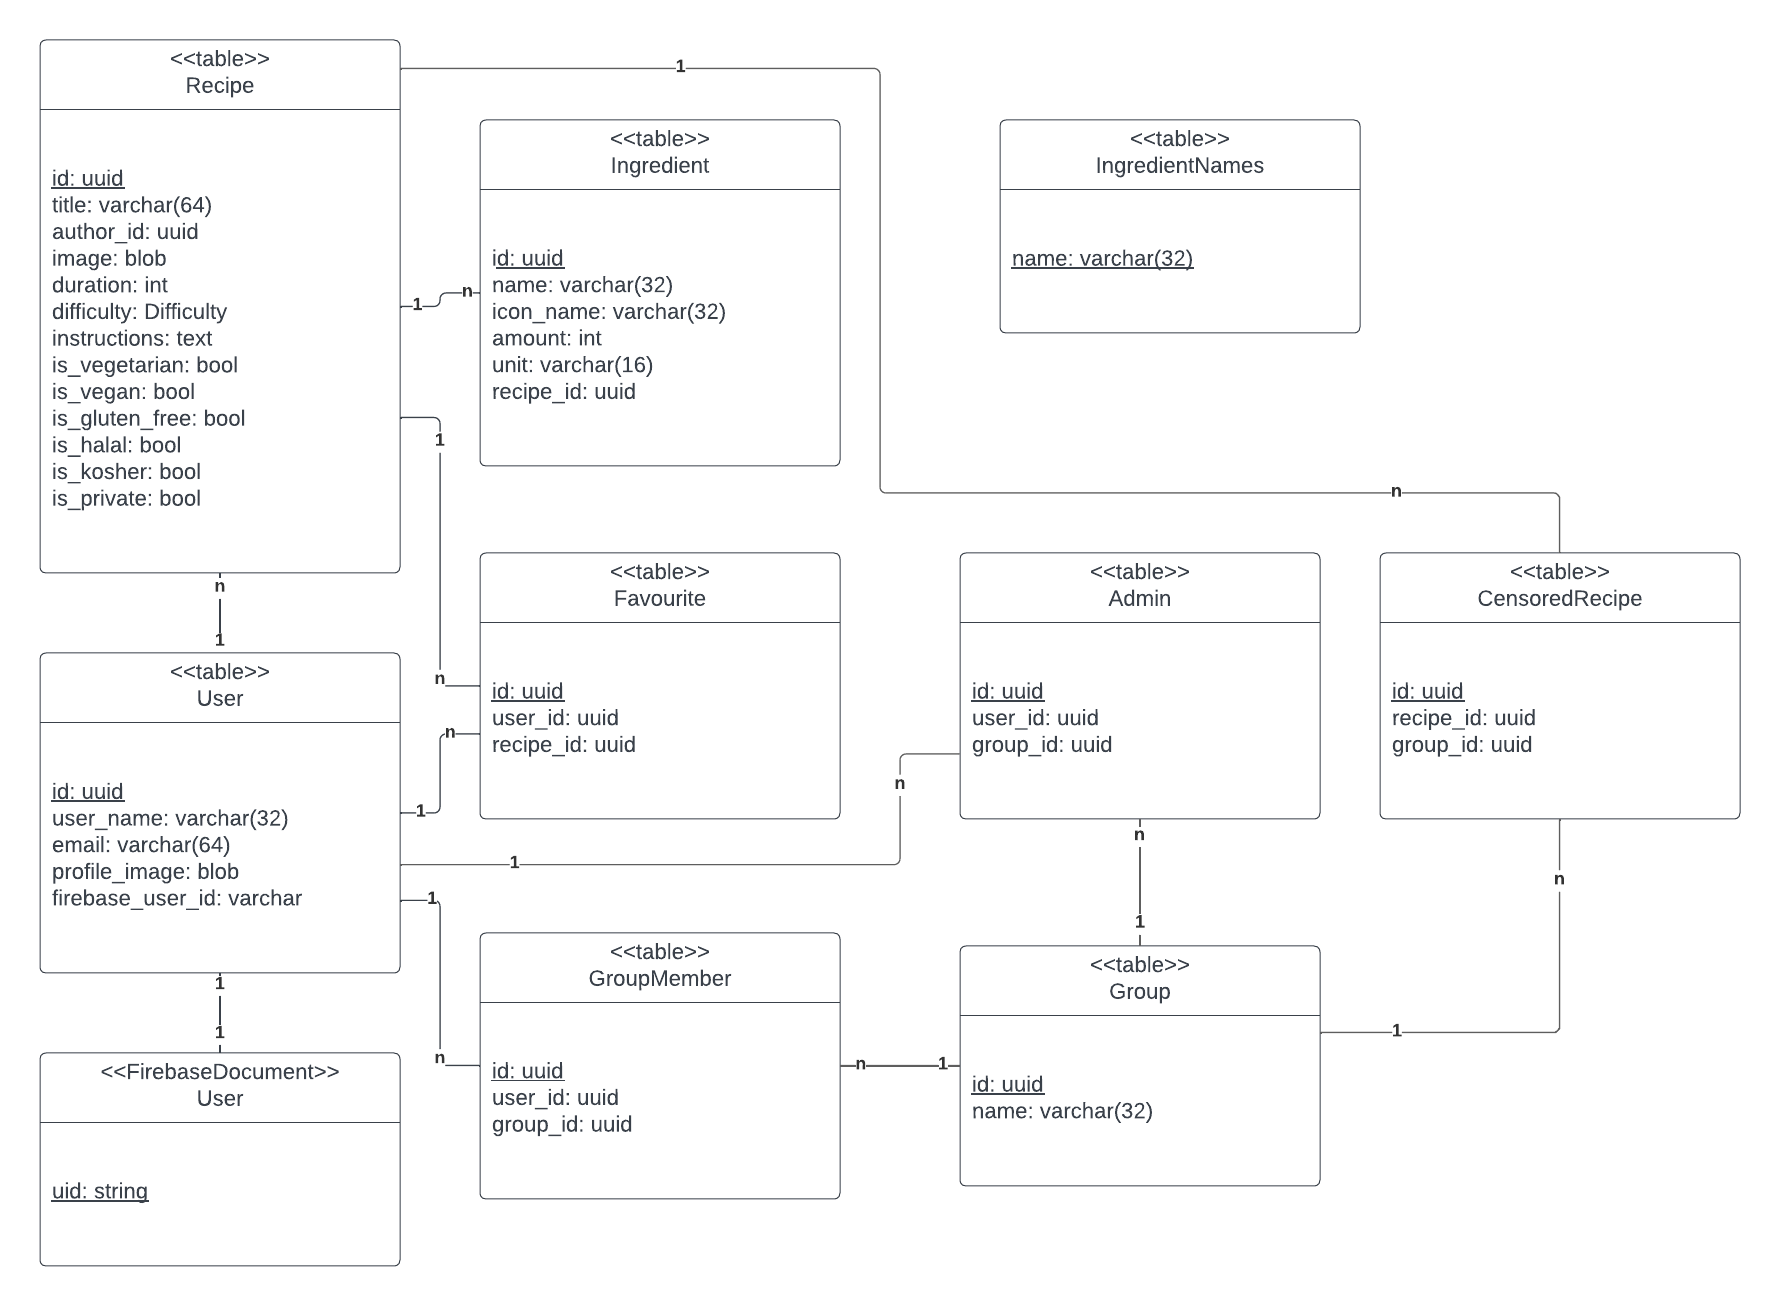
\includegraphics[width = \linewidth]{images/Database/schema.png}
    \caption{Datenbankschema}
\end{figure}
Im Datenbankschema werden die einzelnen Entitäten der App abgebildet. Die einzelnen Tabellen werden nun genauer erläutert.
\newpage
\subsubsection{Recipe}
Die Tabelle "Recipe" enthält die Rezepte und besitzt die folgenden Attribute:
\paragraph{id (uuid - primary key):} Die Id stellt den Primärschlüssel des Rezepts dar und muss daher eindeutig und nicht leer sein. Der Datentyp ist \Gls{uuid}. Sie wird automatisch generiert.
\paragraph{title (varchar(64) - not null):} Der Titel des Rezepts. Der Datentyp ist \Gls{varchar}. Er darf nicht leer und maximal 64 Zeichen lang sein.
\paragraph{author\_id (uuid - not null, foreign key):} Hierbei handelt es sich um die Id des Autors des Rezepts als Fremdschlüssel. Sie darf nicht leer sein und der Datentyp ist \Gls{uuid}, da es sich um eine Id handelt.
\paragraph{image (blob):} Das Bild des Rezepts in binär Code. Der Datentyp ist \Gls{blob}.
\paragraph{duration (int - not null):} Die Zubereitungszeit des Rezepts in Minuten. Der Datentyp ist Integer. Sie darf nicht leer sein.
\paragraph{difficulty (Difficulty - not null):} Die Schwierigkeit des Rezepts, die nicht leer sein darf. Der Datentyp "Difficulty" ist ein Enum, mit den Werten "easy", "medium" und "hard".
\paragraph{instructions (text - not null):} Die Zubereitungsanleitung des Rezepts, die nicht leer sein darf. Der Datentyp ist Text, was einer unbegrenzten Zeichenkette entspricht.
\paragraph{is\_vegetarian (bool - not null):} Gibt an, ob das \Gls{label} "Vegetarisch" aktiviert ist. Der Datentyp ist Boolean und darf nicht leer sein.
\paragraph{is\_vegan (bool - not null):} Gibt an, ob das \Gls{label} "Vegan" aktiviert ist. Der Datentyp ist Boolean und darf nicht leer sein.
\paragraph{is\_gluten\_free (bool - not null):} Gibt an, ob das \Gls{label} "Glutenfrei" aktiviert ist. Der Datentyp ist Boolean und darf nicht leer sein.
\paragraph{is\_halal (bool - not null):} Gibt an, ob das \Gls{label} "Halal" aktiviert ist. Der Datentyp ist Boolean und darf nicht leer sein.
\paragraph{is\_kosher (bool - not null):} Gibt an, ob das \Gls{label} "Koscher" aktiviert ist. Der Datentyp ist Boolean und darf nicht leer sein.
\newpage
\subsubsection{Ingredient}
Die Tabelle "Ingredient" enthält die Zutaten, die den eizelnen Rezepten zugeordnet sind und besitzt die folgenden Attribute:
\paragraph{id (uuid - primary key):} Die Id stellt den Primärschlüssel der Zutat dar und muss daher nicht leer und eindeutig sein. Der Datentyp ist \Gls{uuid}. Sie wird automatisch generiert.
\paragraph{name (varchar(32) - not null):} Der Name der Zutat. Der Datentyp ist \Gls{varchar}. Er darf nicht leer und maximal 32 Zeichen lang sein.
\paragraph{icon\_name (varchar(32))} Der Name des Icons, das die Zutat repräsentiert. Der Datentyp ist \Gls{varchar}. Er ist maximal 32 Zeichen lang.
\paragraph{amount (int - not null):} Die Menge der Zutat in der jeweiligen Einheit. Sie darf nicht leer sein und der Datentyp ist Integer.
\paragraph{unit (varchar(16)):} Die Einheit der Zutat. Der Datentyp ist \Gls{varchar}. Sie ist maximal 16 Zeichen lang und optional.
\paragraph{recipe\_id (uuid - not null, foreign key):} Hierbei handelt es sich um die Id des Rezepts, zu dem die Zutat gehört, als Fremdschlüssel. Sie darf nicht leer sein und der Datentyp ist \Gls{uuid}, da es sich um eine Id handelt.
\newpage
\subsubsection{IngredientNames}
Die Tabelle "IngredientNames" enthält lediglich die Namen der Zutaten, die in der Vorschlagsliste beim Zutaten erstellen angezeigt werden. Sie besitzt die folgenden Attribute:
\paragraph{name (varchar(32) - primary key):} Der Name der Zutat. Der Datentyp ist \Gls{varchar}. Es handelt sich um den Primärschlüssel und der Name muss daher eindeutig und nicht leer sein.
\newpage
\subsubsection{User}
Die Tabelle "User" enthält die Benutzer der App und besitzt die folgenden Attribute:
\paragraph{id (uuid - primary key):} Die Id stellt den Primärschlüssel des Benutzers dar und muss daher eindeutig und nicht leer sein. Der Datentyp ist \Gls{uuid}. Sie wird automatisch generiert.
\paragraph{user\_name (varchar(32) - not null):} Der Benutzername des Benutzers. Der Datentyp ist \Gls{varchar}. Er darf nicht leer und maximal 32 Zeichen lang sein.
\paragraph{email (varchar(64) - not null):} Die E-Mail-Adresse des Benutzers. Der Datentyp ist \Gls{varchar}. Sie darf nicht leer und maximal 64 Zeichen lang sein.
\paragraph{profile\_image (blob):} Das Profilbild des Benutzers in binär Code. Der Datentyp ist \Gls{blob}.
\paragraph{firebase\_user\_id (varchar - not null, unique)} Die Id des Benutzers, die in der Firebase Datenbank hinterlegt ist. Der Datentyp ist \Gls{varchar}. Sie muss eindeutig und nicht leer sein. Sie dient als Fremdschlüssel über die Datenbank hinweg zu Firebase.
\newpage
\subsubsection{Favourite}
Die Tabelle "Favourite" repräsentiert die Many-To-Many-Beziehung zwischen den Benutzern und den Rezepten, die sie favorisiert haben. Sie besitzt die folgenden Attribute:
\paragraph{id (uuid - primary key):} Die Id stellt den Primärschlüssel der Beziehung dar und muss daher eindeutig und nicht leer sein. Der Datentyp ist \Gls{uuid}. Sie wird automatisch generiert.
\paragraph{user\_id (uuid - not null, foreign key):} Hierbei handelt es sich um die Id des Benutzers, der das Rezept favorisiert hat, als Fremdschlüssel. Sie darf nicht leer sein und der Datentyp ist \Gls{uuid}, da es sich um eine Id handelt.
\paragraph{recipe\_id (uuid - not null, foreign key):} Hierbei handelt es sich um die Id des Rezepts, das favorisiert wurde, als Fremdschlüssel. Sie darf nicht leer sein und der Datentyp ist \Gls{uuid}, da es sich um eine Id handelt.
\newpage
\subsubsection{Group}
Die Tabelle "Group" enthält die Gruppen bzw. Squads und besitzt die folgenden Attribute:
\paragraph{id (uuid - primary key):} Die Id stellt den Primärschlüssel der Gruppe dar und muss daher eindeutig und nicht leer sein. Der Datentyp ist \Gls{uuid}. Sie wird automatisch generiert.
\paragraph{name (varchar(32) - not null):} Der Name der Gruppe. Der Datentyp ist \Gls{varchar}. Er darf nicht leer und maximal 32 Zeichen lang sein.
\newpage
\subsubsection{GroupMember}
Die Tabelle "GroupMember" repräsentiert die Many-To-Many-Beziehung zwischen den Gruppen und den Benutzern, die Mitglied der Gruppe sind. Sie besitzt die folgenden Attribute:
\paragraph{id (uuid - primary key):} Die Id stellt den Primärschlüssel der Beziehung dar und muss daher eindeutig und nicht leer sein. Der Datentyp ist \Gls{uuid}. Sie wird automatisch generiert.
\paragraph{user\_id (uuid - not null, foreign key):} Hierbei handelt es sich um die Id des Benutzers, der Mitglied der Gruppe ist, als Fremdschlüssel. Sie darf nicht leer sein und der Datentyp ist \Gls{uuid}, da es sich um eine Id handelt.
\paragraph{group\_id (uuid - not null, foreign key):} Hierbei handelt es sich um die Id der Gruppe, zu der der Benutzer gehört, als Fremdschlüssel. Sie darf nicht leer sein und der Datentyp ist \Gls{uuid}, da es sich um eine Id handelt.
\newpage
\subsubsection{Admin}
Die Tabelle "Admin" repräsentiert die Many-To-Many-Beziehung zwischen den Gruppen und den Benutzern, die Administratoren der Gruppe sind. Sie besitzt die folgenden Attribute:
\paragraph{id (uuid - primary key):} Die Id stellt den Primärschlüssel der Beziehung dar und muss daher eindeutig und nicht leer sein. Der Datentyp ist \Gls{uuid}. Sie wird automatisch generiert.
\paragraph{user\_id (uuid - not null, foreign key):} Hierbei handelt es sich um die Id des Benutzers, der Administrator der Gruppe ist, als Fremdschlüssel. Sie darf nicht leer sein und der Datentyp ist \Gls{uuid}, da es sich um eine Id handelt.
\paragraph{group\_id (uuid - not null, foreign key):} Hierbei handelt es sich um die Id der Gruppe, zu der der Benutzer gehört, als Fremdschlüssel. Sie darf nicht leer sein und der Datentyp ist \Gls{uuid}, da es sich um eine Id handelt.
\newpage
\subsubsection{CensoredRecipe}
Die Tabelle "CensoredRecipe" repräsentiert die Many-To-Many-Beziehung zwischen den Gruppen und den Rezepten, die die jeweiligen Administratoren zensiert haben. Sie besitzt die folgenden Attribute:
\paragraph{id (uuid - primary key):} Die Id stellt den Primärschlüssel der Beziehung dar und muss daher eindeutig und nicht leer sein. Der Datentyp ist \Gls{uuid}. Sie wird automatisch generiert.
\paragraph{recipe\_id (uuid - not null, foreign key):} Hierbei handelt es sich um die Id des Rezepts, das zensiert wurde, als Fremdschlüssel. Sie darf nicht leer sein und der Datentyp ist \Gls{uuid}, da es sich um eine Id handelt.
\paragraph{group\_id (uuid - not null, foreign key):} Hierbei handelt es sich um die Id der Gruppe, zu der der Administrator gehört, als Fremdschlüssel. Sie darf nicht leer sein und der Datentyp ist \Gls{uuid}, da es sich um eine Id handelt.
\newpage

\section{Ablaufbeschreibung}

\section{Klassenindex}
\subsection{Client-Klassen}
\subsection{Server-Klassen}

\section{Glossar}
\printglossary[style=altlist]
\end{document}